\documentclass[8pt]{book}

\usepackage{xeCJK}
\usepackage{listings}
\usepackage{multirow}
\usepackage{longtable}
\usepackage{fontspec}
\usepackage{ctex}
\usepackage[top=3cm,bottom=3cm,left=3cm,right=3cm, headsep=8pt]{geometry} % Page margins
\geometry{papersize={19cm,24cm}}
\usepackage{graphicx} % Required for including pictures
\graphicspath{{Pictures/}{Image/common/}} % Specifies the directory where pictures are stored
\usepackage{lipsum} % Inserts dummy text
\usepackage[ddmmyyyy]{datetime}
\usepackage{pgf}
\usepackage{tikz} % Required for drawing custom shapes
\usetikzlibrary{shapes,arrows,automata,calc}
\usepackage[english]{babel} % English language/hyphenation
\usepackage{enumitem} % Customize lists
\setlist{nolistsep} % Reduce spacing between bullet points and numbered lists
\usepackage{booktabs} % Required for nicer horizontal rules in tables
\usepackage{xcolor} % Required for specifying colors by name
\definecolor{ocre}{RGB}{243,102,25} % Define the orange color used for highlighting throughout the book
\usepackage{avant} % Use the Avantgarde font for headings
%\usepackage{times} % Use the Times font for headings
\usepackage{mathptmx} % Use the Adobe Times Roman as the default text font together with math symbols from the Sym­bol, Chancery and Com­puter Modern fonts
\usepackage{microtype} % Slightly tweak font spacing for aesthetics
\usepackage[T1]{fontenc}
\usepackage[utf8]{inputenc}
{\renewcommand{\bibname}{References}}
%\usepackage[backend=bibtex,style=numeric]{biblatex}
%\defbibheading{bibempty}{}
\usepackage{calc} % 简单的计算功能
\usepackage{makeidx} % 创建索引
\makeindex % Tells LaTeX to create the files required for indexing
\usepackage{titletoc} % 目录操作
\usepackage{verse}
\usepackage[bookmarksopen,bookmarksdepth=4]{hyperref}


\makeatletter
\def\UrlAlphabet{%
	\do\a\do\b\do\c\do\d\do\e\do\f\do\g\do\h\do\i\do\j%
	\do\k\do\l\do\m\do\n\do\o\do\p\do\q\do\r\do\s\do\t%
	\do\u\do\v\do\w\do\x\do\y\do\z\do\A\do\B\do\C\do\D%
	\do\E\do\F\do\G\do\H\do\I\do\J\do\K\do\L\do\M\do\N%
	\do\O\do\P\do\Q\do\R\do\S\do\T\do\U\do\V\do\W\do\X%
	\do\Y\do\Z}
\def\UrlDigits{\do\1\do\2\do\3\do\4\do\5\do\6\do\7\do\8\do\9\do\0}
\g@addto@macro{\UrlBreaks}{\UrlOrds}
\g@addto@macro{\UrlBreaks}{\UrlAlphabet}
\g@addto@macro{\UrlBreaks}{\UrlDigits}
\makeatother


%When compile under liunx% 

%\setCJKmainfont{WenQuanYi Micro Hei} % 设置缺省中文字体

\contentsmargin{0cm} % Removes the default margin

\lstdefinelanguage
   [x64]{Assembler}     % add a "x64" dialect of Assembler
   [x86masm]{Assembler} % based on the "x86masm" dialect
   % with these extra keywords:
   {morekeywords={CDQE,CQO,CMPSQ,CMPXCHG16B,JRCXZ,LODSQ,MOVSXD, %
                  POPFQ,PUSHFQ,SCASQ,STOSQ,IRETQ,RDTSCP,SWAPGS, %
                  rax,rdx,rcx,rbx,rsi,rdi,rsp,rbp, %
                  r8,r8d,r8w,r8b,r9,r9d,r9w,r9b, %
                  r10,r10d,r10w,r10b,r11,r11d,r11w,r11b, %
                  r12,r12d,r12w,r12b,r13,r13d,r13w,r13b, %
                  r14,r14d,r14w,r14b,r15,r15d,r15w,r15b}} % etc.

\lstdefinelanguage{JavaScript}{
	keywords={typeof, new, true, false, catch, function, return, null, catch, switch, var, if, in, while, do, else, case, break},
	keywordstyle=\color{blue}\bfseries,
	ndkeywords={class, export, boolean, throw, implements, import, this},
	ndkeywordstyle=\color{darkgray}\bfseries,
	identifierstyle=\color{black},
	sensitive=false,
	comment=[l]{//},
	morecomment=[s]{/*}{*/},
	commentstyle=\color{purple}\ttfamily,
	stringstyle=\color{red}\ttfamily,
	morestring=[b]',
	morestring=[b]"
}

%Figure显示为中文的“图”
\renewcommand\figurename{图}

\newcommand{\cndash}{\rule{0.2em}{0pt}\rule[0.35em]{1.6em}{0.05em}\rule{0.2em}{0pt}}

\setcounter{tocdepth}{2}

%Set Code Format%
\lstloadlanguages{C, csh, make,python,Java,JavaScript,ACM,Haskell,[x64]Assembler}
\lstset{	  
	alsolanguage= XML,  
	tabsize=4, %  
	frame=shadowbox, %把代码用带有阴影的框圈起来  
	commentstyle=\color{red!50!green!50!blue!50},%浅灰色的注释
	frameround=tttt,  
	rulesepcolor=\color{red!20!green!20!blue!20},%代码块边框为淡青色  
	keywordstyle=\color{blue!90}\bfseries, %代码关键字的颜色为蓝色,粗体  
	showstringspaces=false,%不显示代码字符串中间的空格标记  
	stringstyle=\ttfamily, % 代码字符串的特殊格式  
	keepspaces=true, %  
	breakindent=22pt, % 
	breaklines=true,%设置代码自动换行 
	numbers=left,%左侧显示行号 往左靠,还可以为right,或none,即不加行号  
	stepnumber=1,%若设置为2,则显示行号为1,3,5,即stepnumber为公差,默认stepnumber=1  
	%numberstyle=\tiny, %行号字体用小号  
	numberstyle={\color[RGB]{0,192,192}\tiny},%设置行号的大小,大小有tiny,scriptsize,footnotesize,small,normalsize,large等  
	numbersep=8pt,  %设置行号与代码的距离,默认是5pt  
	basicstyle=\ttfamily, % 这句设置代码的大小  
	showspaces=false, % 
	escapechar=`,
	flexiblecolumns=true, %  
	breaklines=true, %对过长的代码自动换行  
	breakautoindent=true,%  
	breakindent=4em, %  	   
	aboveskip=1em, %代码块边框  
	tabsize=4,  
	showstringspaces=false, %不显示字符串中的空格  
	backgroundcolor=\color[RGB]{245,245,244},   %代码背景色  
	%backgroundcolor=\color[rgb]{0.91,0.91,0.91}    %添加背景色  
	escapeinside={``}{\_},  %在``里显示中文  
	%% added by http://bbs.ctex.org/viewthread.php?tid=53451  
	fontadjust,  
	captionpos=t,  
	framextopmargin=2pt,
	framexbottommargin=2pt,
	abovecaptionskip=-3pt,
	belowcaptionskip=3pt,  
	xleftmargin=1em,
	xrightmargin=1em, % 设定listing左右的空白  
	texcl=true
}

% Part text styling
%%%\titlecontents{part}[0cm]{\addvspace{20pt}\centering\large\sffamily}{}{}{}

% Chapter text styling
\titlecontents{chapter}[1.25cm] % Indentation
{\addvspace{12pt}\large\sffamily\bfseries} % Spacing and font options for chapters
{\color{ocre!60}\contentslabel[\Large\thecontentslabel]{1.25cm}\color{ocre}} % Chapter number
{\color{ocre}}  
{\color{ocre!60}\normalsize\;\titlerule*[.5pc]{.}\;\thecontentspage} % Page number

% Section text styling
\titlecontents{section}[1.25cm] % Indentation
{\addvspace{3pt}\sffamily\bfseries} % Spacing and font options for sections
{\contentslabel[\thecontentslabel]{1.25cm}} % Section number
{}
{\hfill\color{black}\thecontentspage} % Page number
[]

% Subsection text styling
\titlecontents{subsection}[1.25cm] % Indentation
{\addvspace{1pt}\sffamily\small} % Spacing and font options for subsections
{\contentslabel[\thecontentslabel]{1.25cm}} % Subsection number
{}
{\ \titlerule*[.5pc]{.}\;\thecontentspage} % Page number
[]

% List of figures
\titlecontents{figure}[0em]
{\addvspace{-5pt}\sffamily}
{\thecontentslabel\hspace*{1em}}
{}
{\ \titlerule*[.5pc]{.}\;\thecontentspage}
[]

% List of tables
\titlecontents{table}[0em]
{\addvspace{-5pt}\sffamily}
{\thecontentslabel\hspace*{1em}}
{}
{\ \titlerule*[.5pc]{.}\;\thecontentspage}
[]

%----------------------------------------------------------------------------------------
%	MINI TABLE OF CONTENTS IN PART HEADS
%----------------------------------------------------------------------------------------

% Chapter text styling
\titlecontents{lchapter}[0em] % Indenting
{\addvspace{15pt}\large\sffamily\bfseries} % Spacing and font options for chapters
{\color{ocre}\contentslabel[\Large\thecontentslabel]{1.25cm}\color{ocre}} % Chapter number
{}  
{\color{ocre}\normalsize\sffamily\bfseries\;\titlerule*[.5pc]{.}\;\thecontentspage} % Page number

% Section text styling
\titlecontents{lsection}[0em] % Indenting
{\sffamily\small} % Spacing and font options for sections
{\contentslabel[\thecontentslabel]{1.25cm}} % Section number
{}
{}

% Subsection text styling
\titlecontents{lsubsection}[.5em] % Indentation
{\normalfont\footnotesize\sffamily} % Font settings
{}
{}
{}

%----------------------------------------------------------------------------------------
%	PAGE HEADERS
%----------------------------------------------------------------------------------------

\usepackage{fancyhdr} % Required for header and footer configuration

\pagestyle{fancy}
\renewcommand{\chaptermark}[1]{\markboth{\sffamily\normalsize\bfseries\chaptername\ \thechapter.\ #1}{}} % Chapter text font settings
\renewcommand{\sectionmark}[1]{\markright{\sffamily\normalsize\thesection\hspace{5pt}#1}{}} % Section text font settings
\fancyhf{} \fancyhead[LE,RO]{\sffamily\normalsize\thepage} % Font setting for the page number in the header
\fancyhead[LO]{\rightmark} % Print the nearest section name on the left side of odd pages
\fancyhead[RE]{\leftmark} % Print the current chapter name on the right side of even pages
\renewcommand{\headrulewidth}{0.5pt} % Width of the rule under the header
\addtolength{\headheight}{2.5pt} % Increase the spacing around the header slightly
\renewcommand{\footrulewidth}{0pt} % Removes the rule in the footer
\fancypagestyle{plain}{\fancyhead{}\renewcommand{\headrulewidth}{0pt}} % Style for when a plain pagestyle is specified

% Removes the header from odd empty pages at the end of chapters
\makeatletter
\renewcommand{\cleardoublepage}{
	\clearpage\ifodd\c@page\else
	\hbox{}
	\vspace*{\fill}
	\thispagestyle{empty}
	\newpage
	\fi}

%----------------------------------------------------------------------------------------
%	THEOREM STYLES
%----------------------------------------------------------------------------------------

\usepackage{amsmath,amsfonts,amssymb,amsthm} % For math equations, theorems, symbols, etc

\newcommand{\intoo}[2]{\mathopen{]}#1\,;#2\mathclose{[}}
\newcommand{\ud}{\mathop{\mathrm{{}d}}\mathopen{}}
\newcommand{\intff}[2]{\mathopen{[}#1\,;#2\mathclose{]}}
\newtheorem{notation}{Notation}[chapter]

% Boxed/framed environments
\newtheoremstyle{ocrenumbox}% % Theorem style name
{0pt}% Space above
{0pt}% Space below
{\normalfont}% % Body font
{}% Indent amount
{\small\bf\sffamily\color{ocre}}% % Theorem head font
{\;}% Punctuation after theorem head
{0.25em}% Space after theorem head
{\small\sffamily\color{ocre}\thmname{#1}\nobreakspace\thmnumber{\@ifnotempty{#1}{}\@upn{#2}}% Theorem text (e.g. Theorem 2.1)
	\thmnote{\nobreakspace\the\thm@notefont\sffamily\bfseries\color{black}---\nobreakspace#3.}} % Optional theorem note
\renewcommand{\qedsymbol}{$\blacksquare$}% Optional qed square

\newtheoremstyle{blacknumex}% Theorem style name
{5pt}% Space above
{5pt}% Space below
{\normalfont}% Body font
{} % Indent amount
{\small\bf\sffamily}% Theorem head font
{\;}% Punctuation after theorem head
{0.25em}% Space after theorem head
{\small\sffamily{\tiny\ensuremath{\blacksquare}}\nobreakspace\thmname{#1}\nobreakspace\thmnumber{\@ifnotempty{#1}{}\@upn{#2}}% Theorem text (e.g. Theorem 2.1)
	\thmnote{\nobreakspace\the\thm@notefont\sffamily\bfseries---\nobreakspace#3.}}% Optional theorem note

\newtheoremstyle{blacknumbox} % Theorem style name
{0pt}% Space above
{0pt}% Space below
{\normalfont}% Body font
{}% Indent amount
{\small\bf\sffamily}% Theorem head font
{\;}% Punctuation after theorem head
{0.25em}% Space after theorem head
{\small\sffamily\thmname{#1}\nobreakspace\thmnumber{\@ifnotempty{#1}{}\@upn{#2}}% Theorem text (e.g. Theorem 2.1)
	\thmnote{\nobreakspace\the\thm@notefont\sffamily\bfseries---\nobreakspace#3.}}% Optional theorem note

% Non-boxed/non-framed environments
\newtheoremstyle{ocrenum}% % Theorem style name
{5pt}% Space above
{5pt}% Space below
{\normalfont}% % Body font
{}% Indent amount
{\small\bf\sffamily\color{ocre}}% % Theorem head font
{\;}% Punctuation after theorem head
{0.25em}% Space after theorem head
{\small\sffamily\color{ocre}\thmname{#1}\nobreakspace\thmnumber{\@ifnotempty{#1}{}\@upn{#2}}% Theorem text (e.g. Theorem 2.1)
	\thmnote{\nobreakspace\the\thm@notefont\sffamily\bfseries\color{black}---\nobreakspace#3.}} % Optional theorem note
\renewcommand{\qedsymbol}{$\blacksquare$}% Optional qed square
\makeatother 

% Defines the theorem text style for each type of theorem to one of the three styles above
\newcounter{dummy} 
\numberwithin{dummy}{section}
\theoremstyle{ocrenumbox}
\newtheorem{theoremeT}[dummy]{Theorem}
\newtheorem{problem}{Problem}[chapter]
\newtheorem{exerciseT}{Exercise}[chapter]
\theoremstyle{blacknumex}
\newtheorem{exampleT}{Example}[chapter]
\theoremstyle{blacknumbox}
\newtheorem{vocabulary}{Vocabulary}[chapter]
\newtheorem{definitionT}{Definition}[section]
\newtheorem{corollaryT}[dummy]{Corollary}
\theoremstyle{ocrenum}
\newtheorem{proposition}[dummy]{Proposition}

%----------------------------------------------------------------------------------------
%	DEFINITION OF COLORED BOXES
%----------------------------------------------------------------------------------------

\RequirePackage[framemethod=default]{mdframed} % Required for creating the theorem, definition, exercise and corollary boxes

% Theorem box
\newmdenv[skipabove=7pt,
skipbelow=7pt,
backgroundcolor=black!5,
linecolor=ocre,
innerleftmargin=5pt,
innerrightmargin=5pt,
innertopmargin=5pt,
leftmargin=0cm,
rightmargin=0cm,
innerbottommargin=5pt]{tBox}

% Exercise box	  
\newmdenv[skipabove=7pt,
skipbelow=7pt,
rightline=false,
leftline=true,
topline=false,
bottomline=false,
backgroundcolor=ocre!10,
linecolor=ocre,
innerleftmargin=5pt,
innerrightmargin=5pt,
innertopmargin=5pt,
innerbottommargin=5pt,
leftmargin=0cm,
rightmargin=0cm,
linewidth=4pt]{eBox}	

% Definition box
\newmdenv[skipabove=7pt,
skipbelow=7pt,
rightline=false,
leftline=true,
topline=false,
bottomline=false,
linecolor=ocre,
innerleftmargin=5pt,
innerrightmargin=5pt,
innertopmargin=0pt,
leftmargin=0cm,
rightmargin=0cm,
linewidth=4pt,
innerbottommargin=0pt]{dBox}	

% Corollary box
\newmdenv[skipabove=7pt,
skipbelow=7pt,
rightline=false,
leftline=true,
topline=false,
bottomline=false,
linecolor=gray,
backgroundcolor=black!5,
innerleftmargin=5pt,
innerrightmargin=5pt,
innertopmargin=5pt,
leftmargin=0cm,
rightmargin=0cm,
linewidth=4pt,
innerbottommargin=5pt]{cBox}

% Creates an environment for each type of theorem and assigns it a theorem text style from the "Theorem Styles" section above and a colored box from above
\newenvironment{theorem}{\begin{tBox}\begin{theoremeT}}{\end{theoremeT}\end{tBox}}
\newenvironment{exercise}{\begin{eBox}\begin{exerciseT}}{\hfill{\color{ocre}\tiny\ensuremath{\blacksquare}}\end{exerciseT}\end{eBox}}				  
\newenvironment{definition}{\begin{dBox}\begin{definitionT}}{\end{definitionT}\end{dBox}}	
\newenvironment{example}{\begin{exampleT}}{\hfill{\tiny\ensuremath{\blacksquare}}\end{exampleT}}		
\newenvironment{corollary}{\begin{cBox}\begin{corollaryT}}{\end{corollaryT}\end{cBox}}	

%----------------------------------------------------------------------------------------
%	REMARK ENVIRONMENT
%----------------------------------------------------------------------------------------

\newenvironment{remark}{\par\vspace{10pt}\small % Vertical white space above the remark and smaller font size
	\begin{list}{}{
			\leftmargin=35pt % Indentation on the left
			\rightmargin=25pt}\item\ignorespaces % Indentation on the right
		\makebox[-2.5pt]{\begin{tikzpicture}[overlay]
			\node[draw=ocre!60,line width=1pt,circle,fill=ocre!25,font=\sffamily\bfseries,inner sep=2pt,outer sep=0pt] at (-15pt,0pt){\textcolor{ocre}{R}};\end{tikzpicture}} % Orange R in a circle
		\advance\baselineskip -1pt}{\end{list}\vskip5pt} % Tighter line spacing and white space after remark

%----------------------------------------------------------------------------------------
%	SECTION NUMBERING IN THE MARGIN
%----------------------------------------------------------------------------------------

\makeatletter
\renewcommand{\@seccntformat}[1]{\llap{\textcolor{ocre}{\csname the#1\endcsname}\hspace{1em}}}                    
\renewcommand{\section}{\@startsection{section}{1}{\z@}
	{-4ex \@plus -1ex \@minus -.4ex}
	{1ex \@plus.2ex }
	{\normalfont\large\sffamily\bfseries}}
\renewcommand{\subsection}{\@startsection {subsection}{2}{\z@}
	{-3ex \@plus -0.1ex \@minus -.4ex}
	{0.5ex \@plus.2ex }
	{\normalfont\sffamily\bfseries}}
\renewcommand{\subsubsection}{\@startsection {subsubsection}{3}{\z@}
	{-2ex \@plus -0.1ex \@minus -.2ex}
	{.2ex \@plus.2ex }
	{\normalfont\small\sffamily\bfseries}}                        
\renewcommand\paragraph{\@startsection{paragraph}{4}{\z@}
	{-2ex \@plus-.2ex \@minus .2ex}
	{.1ex}
	{\normalfont\small\sffamily\bfseries}}

%----------------------------------------------------------------------------------------
%	PART HEADINGS
%----------------------------------------------------------------------------------------

% numbered part in the table of contents
\newcommand{\@mypartnumtocformat}[2]{%
	\setlength\fboxsep{0pt}%
	\noindent\colorbox{ocre!20}{\strut\parbox[c][.7cm]{\ecart}{\color{ocre!70}\Large\sffamily\bfseries\centering#1}}\hskip\esp\colorbox{ocre!40}{\strut\parbox[c][.7cm]{\linewidth-\ecart-\esp}{\Large\sffamily\centering#2}}}%
%%%%%%%%%%%%%%%%%%%%%%%%%%%%%%%%%%
% unnumbered part in the table of contents
\newcommand{\@myparttocformat}[1]{%
	\setlength\fboxsep{0pt}%
	\noindent\colorbox{ocre!40}{\strut\parbox[c][.7cm]{\linewidth}{\Large\sffamily\centering#1}}}%
%%%%%%%%%%%%%%%%%%%%%%%%%%%%%%%%%%
\newlength\esp
\setlength\esp{4pt}
\newlength\ecart
\setlength\ecart{1.2cm-\esp}
\newcommand{\thepartimage}{}%
\newcommand{\partimage}[1]{\renewcommand{\thepartimage}{#1}}%

\def\@part[#1]#2{%
	\ifnum \c@secnumdepth >-2\relax%
	\refstepcounter{part}%
	\addcontentsline{toc}{part}{\texorpdfstring{\protect\@mypartnumtocformat{\thepart}{#1}}{\partname~\thepart\ ---\ #1}}
	\else%
	\addcontentsline{toc}{part}{\texorpdfstring{\protect\@myparttocformat{#1}}{#1}}%
	\fi%
	\startcontents%
	\markboth{}{}%
	{\thispagestyle{empty}%
		\begin{tikzpicture}[remember picture,overlay]%
		\node at (current page.north west){\begin{tikzpicture}[remember picture,overlay]%	
			\fill[ocre!20](0cm,0cm) rectangle (\paperwidth,-\paperheight);
			\node[anchor=north] at (4cm,-3.25cm){\color{ocre!40}\fontsize{220}{100}\sffamily\bfseries\@Roman\c@part}; 
			\node[anchor=south east] at (\paperwidth-1cm,-\paperheight+1cm){\parbox[t][][t]{8.5cm}{
					\printcontents{l}{0}{\setcounter{tocdepth}{1}}%
			}};
			\node[anchor=north east] at (\paperwidth-1.5cm,-3.25cm){\parbox[t][][t]{15cm}{\strut\raggedleft\color{white}\fontsize{30}{30}\sffamily\bfseries#2}};\end{tikzpicture}};
	\end{tikzpicture}}
\@endpart}

\def\@spart#1{%
\startcontents%
\phantomsection
{\thispagestyle{empty}%
	\begin{tikzpicture}[remember picture,overlay]%
	\node at (current page.north west){\begin{tikzpicture}[remember picture,overlay]%	
		\fill[ocre!20](0cm,0cm) rectangle (\paperwidth,-\paperheight);
		\node[anchor=north east] at (\paperwidth-1.5cm,-3.25cm){\parbox[t][][t]{15cm}{\strut\raggedleft\color{white}\fontsize{30}{30}\sffamily\bfseries#1}};
		\end{tikzpicture}};
\end{tikzpicture}}
\addcontentsline{toc}{part}{\texorpdfstring{%
	\setlength\fboxsep{0pt}%
	\noindent\protect\colorbox{ocre!40}{\strut\protect\parbox[c][.7cm]{\linewidth}{\Large\sffamily\protect\centering #1\quad\mbox{}}}}{#1}}%
\@endpart}
\def\@endpart{\vfil\newpage
\if@twoside
\if@openright
\null
\thispagestyle{empty}%
\newpage
\fi
\fi
\if@tempswa
\twocolumn
\fi}

%----------------------------------------------------------------------------------------
%	CHAPTER HEADINGS
%----------------------------------------------------------------------------------------

% A switch to conditionally include a picture, implemented by  Christian Hupfer
\newif\ifusechapterimage
\usechapterimagetrue
\newcommand{\thechapterimage}{}%
\newcommand{\chapterimage}[1]{\ifusechapterimage\renewcommand{\thechapterimage}{#1}\fi}%
\def\@makechapterhead#1{%
{\parindent \z@ \raggedright \normalfont
\ifnum \c@secnumdepth >\m@ne
\if@mainmatter
\begin{tikzpicture}[remember picture,overlay]
\node at (current page.north west)
{\begin{tikzpicture}[remember picture,overlay]
	\node[anchor=north west,inner sep=0pt] at (0,0) {\ifusechapterimage\includegraphics[width=\paperwidth]{\thechapterimage}\fi};
	\draw[anchor=west] (\Gm@lmargin,-9cm) node [line width=2pt,rounded corners=15pt,draw=ocre,fill=white,fill opacity=0.5,inner sep=15pt]{\strut\makebox[22cm]{}};
	\draw[anchor=west] (\Gm@lmargin+.3cm,-9cm) node {\huge\sffamily\bfseries\color{black}\thechapter. #1\strut};
	\end{tikzpicture}};
\end{tikzpicture}
\else
\begin{tikzpicture}[remember picture,overlay]
\node at (current page.north west)
{\begin{tikzpicture}[remember picture,overlay]
\node[anchor=north west,inner sep=0pt] at (0,0) {\ifusechapterimage\includegraphics[width=\paperwidth]{\thechapterimage}\fi};
\draw[anchor=west] (\Gm@lmargin,-9cm) node [line width=2pt,rounded corners=15pt,draw=ocre,fill=white,fill opacity=0.5,inner sep=15pt]{\strut\makebox[22cm]{}};
\draw[anchor=west] (\Gm@lmargin+.3cm,-9cm) node {\huge\sffamily\bfseries\color{black}#1\strut};
\end{tikzpicture}};
\end{tikzpicture}
\fi\fi\par\vspace*{270\p@}}}

%-------------------------------------------

\def\@makeschapterhead#1{%
\begin{tikzpicture}[remember picture,overlay]
\node at (current page.north west)
{\begin{tikzpicture}[remember picture,overlay]
\node[anchor=north west,inner sep=0pt] at (0,0) {\ifusechapterimage\includegraphics[width=\paperwidth]{\thechapterimage}\fi};
\draw[anchor=west] (\Gm@lmargin,-9cm) node [line width=2pt,rounded corners=15pt,draw=ocre,fill=white,fill opacity=0.5,inner sep=15pt]{\strut\makebox[22cm]{}};
\draw[anchor=west] (\Gm@lmargin+.3cm,-9cm) node {\huge\sffamily\bfseries\color{black}#1\strut};
\end{tikzpicture}};
\end{tikzpicture}
\par\vspace*{270\p@}}
\makeatother

%----------------------------------------------------------------------------------------
%	HYPERLINKS IN THE DOCUMENTS
%----------------------------------------------------------------------------------------

\usepackage{hyperref}
\hypersetup{hidelinks,backref=true,pagebackref=true,hyperindex=true,colorlinks=false,breaklinks=true,urlcolor= ocre,bookmarks=true,bookmarksopen=false,pdftitle={Title},pdfauthor={Author}}
\usepackage{bookmark}
\bookmarksetup{
open,
numbered,
addtohook={%
\ifnum\bookmarkget{level}=0 % chapter
\bookmarksetup{bold}%
\fi
\ifnum\bookmarkget{level}=-1 % part
\bookmarksetup{color=ocre,bold}%
\fi
}
}

%\addbibresource{Bronvermelding.bib} 

\begin{document}

\begingroup
\thispagestyle{empty}
\begin{tikzpicture}[remember picture,overlay]
\coordinate [below=12cm] (midpoint) at (current page.north);
\node at (current page.north west)
{\begin{tikzpicture}[remember picture,overlay]
\node[anchor=north west,inner sep=0pt] at (0,0) {
\includegraphics[width=\paperwidth]{background}}; % Background image
\draw[anchor=north] (midpoint) node [fill=ocre!30!white,fill opacity=0.6,text opacity=1,inner sep=1cm]{\Huge\centering\bfseries\sffamily\parbox[c][][t]{\paperwidth}{\centering Kubernetes \\[15pt] % Book title
{\Large 注解}\\[20pt] % Subtitle
{\large Dolphin}}}; % Author name
\end{tikzpicture}};
\end{tikzpicture}
\vfill
\endgroup


%----------------------------------------------------------------------------------------
%	BLANK PAGE
%----------------------------------------------------------------------------------------

\newpage
~\vfill
\thispagestyle{empty}

%----------------------------------------------------------------------------------------
%	COPYRIGHT PAGE
%----------------------------------------------------------------------------------------

\newpage
~\vfill
\thispagestyle{empty}

\noindent Copyright \textcopyright\ 2017 Xiaoqiang Jiang\\ % Copyright notice

\noindent \textsc{Edited by Xiaoqiang Jiang}\\ % Publisher

\noindent \textsc{\url{http://jiangxiaoqiang.github.com/}}\\

\noindent All Rights Reserved.\\ % License information

\noindent \textit{Version \currenttime, \today} % Printing/edition date


%----------------------------------------------------------------------------------------
%	TABLE OF CONTENTS
%----------------------------------------------------------------------------------------

%\usechapterimagefalse % If you don't want to include a chapter image, use this to toggle images off - it can be enabled later with \usechapterimagetrue

\chapterimage{chapterhead1.pdf} % Table of contents heading image

\pagestyle{empty} % No headers

\tableofcontents % Print the table of contents itself

\cleardoublepage % Forces the first chapter to start on an odd page so it's on the right

\pagestyle{fancy} % Print headers again

%----------------------------------------------------------------------------------------
%	BLANK PAGE
%----------------------------------------------------------------------------------------

参考资料\url{https://zh.wikisource.org/zh/%E8%A9%A9%E7%B6%93}:


\mainmatter

%----------------------------------------------------------------------------------------
% PART
%----------------------------------------------------------------------------------------


\part{风}

%----------------------------------------------------------------------------------------
%	CHAPTER 1
%----------------------------------------------------------------------------------------

\chapterimage{chapterhead2.pdf} % Chapter heading image

\chapter{Kubernetes基础}

\section{Kubernetes部署}

部署Kubernetes最难的点是获取部署文件,这个问题解决了,其他问题就都顺利了。Kubernetes是Google基于Borg开源的容器编排调度引擎,作为CNCF(Cloud Native Computing Foundation)最重要的组件之一,它的目标不仅仅是一个编排系统,而是提供一个规范,可以让你来描述集群的架构,定义服务的最终状态,Kubernetes可以帮你将系统自动地达到和维持在这个状态。安装步骤来源于handbook\footnote{参考地址:\url{https://jimmysong.io/kubernetes-handbook/practice/create-tls-and-secret-key.html}}。后来发现Kubernetes官方文档\footnote{\url{https://kubernetes.io/zh/docs/concepts/cluster-administration/certificates/}}描述更详细、更清晰。 还可以参考Kubernetes交互式部署手册\footnote{\url{https://kubernetes.io/docs/tutorials/kubernetes-basics/deploy-app/deploy-interactive/}}。


\begin{table}[htbp]
	\caption{组件分布}
	\label{table:ca}
	\begin{center}
		\begin{tabular}{|c|c|p{7cm}|}
			\hline
			\multirow{1}{*}{主机}
			& \multicolumn{1}{c|}{角色}
			& \multicolumn{1}{c|}{组件}\\			
			\cline{1-3}
			172.19.104.231 & k8s master & etcd,kube-apiserver,kube-controller-manager,kube-scheduler  \\
			\hline
			172.19.104.230 & k8s node01  &  docker,kubelet,kube-proxy  \\
			\hline
			172.19.150.82 & k8s node02  &  docker,kubelet,kube-proxy  \\
			\hline						
		\end{tabular}	
	\end{center}
\end{table}

定义整个kubernetes集群都需要使用到的环境变量(Environment Variable)\footnote{来源地址:\url{https://github.com/opsnull/follow-me-install-kubernetes-cluster}}:

\begin{lstlisting}[language=Bash]
#!/usr/bin/bash

# 生成EncryptionConfig所需的加密key
export ENCRYPTION_KEY=$(head -c 32 /dev/urandom | base64)

# 集群各机器IP数组
export NODE_IPS=(172.19.104.231 172.19.104.230 172.19.150.82)

# 集群各IP对应的主机名数组
# Azshara是游戏《魔兽世界》中的角色
export NODE_NAMES=(azshara-k8s01 azshara-k8s02 azshara-k8s03)

# etcd集群服务地址列表
export ETCD_ENDPOINTS="https://172.19.104.231:2379,https://172.19.104.230:2379,https://172.19.150.82:2379"

# etcd集群间通信的IP和端口
export ETCD_NODES="azshara-k8s01=https://172.19.104.231:2380,azshara-k8s02=https://172.19.104.230:2380,azshara-k8s03=https://172.19.150.82:2380"

# kube-apiserver的反向代理(kube-nginx)地址端口
export KUBE_APISERVER="https://127.0.0.1:8443"

# 节点间互联网络接口名称
export IFACE="eth0"

# etcd数据目录
export ETCD_DATA_DIR="/opt/k8s/etcd/data"

# etcd WAL目录,建议是SSD磁盘分区
# 或者和ETCD\_DATA\_DIR不同的磁盘分区
export ETCD_WAL_DIR="/opt/k8s/etcd/wal"

# k8s各组件数据目录
export K8S_DIR="/opt/k8s/k8s"

# docker数据目录
export DOCKER_DIR="/opt/k8s/docker"

# 以下参数一般不需要修改

# TLS Bootstrapping使用的Token
# 可以使用命令head -c 16 /dev/urandom|od -An -t x|tr -d ' '生成
BOOTSTRAP_TOKEN="41f7e4ba8b7be874fcff18bf5cf41a7c"

# 最好使用当前未用的网段来定义服务网段和Pod网段

# 服务网段,部署前路由不可达,部署后集群内路由可达(kube-proxy保证)
SERVICE_CIDR="10.254.0.0/16"

# Pod网段,建议/16段地址
# 部署前路由不可达,部署后集群内路由可达(flanneld保证)
CLUSTER_CIDR="172.30.0.0/16"

# 服务端口范围(NodePort Range)
export NODE_PORT_RANGE="30000-32767"

# flanneld网络配置前缀
export FLANNEL_ETCD_PREFIX="/kubernetes/network"

# kubernetes服务IP(一般是SERVICE\_CIDR中第一个IP)
export CLUSTER_KUBERNETES_SVC_IP="10.254.0.1"

# 集群DNS服务IP(从SERVICE\_CIDR中预分配)
export CLUSTER_DNS_SVC_IP="10.254.0.2"

# 集群DNS域名(末尾不带点号)
export CLUSTER_DNS_DOMAIN="cluster.local"

# 将二进制目录/opt/k8s/bin加到PATH中
export PATH=/opt/k8s/bin:$PATH
\end{lstlisting}

这里设置数据目录时,如果是多主机挂载的同一个磁盘,那么数据目录就不能够放在这个挂载的磁盘下,原因很简单,后面等于多个主机的数据放在一个目录下,会冲突,除非确定这个数据只有一个主机会用到。因为用阿里云挂载的数据盘很大,开始时,将etcd的数据文件放在data目录(data目录挂载的一个500GB的数据盘)下,深深的为自己的高瞻远瞩和机制折服,后面etcd启动的时候总是提示文件锁定,更奇怪的是启动了a节点,b节点宕掉了,百撕不得其解。还好反应过来了,否则不知道要掉坑里多久。调整环境变量中的路径,重新运行脚本生成服务即可。


\subsubsection{创建TLS证书和秘钥}


\paragraph{安装证书创建工具CFSSL}

生成证书可以通过easyrsa、openssl或cfssl生成证书。创建传输层安全TLS(Transport Layer Security)证书和密钥在服务器172.19.104.231上进行。直接使用二进制源码包安装CFSSL(CloudFlare Secure Sockets Layer):

\begin{lstlisting}[language=Bash]
wget https://pkg.cfssl.org/R1.2/cfssl_linux-amd64
chmod +x cfssl_linux-amd64
mv cfssl_linux-amd64 /usr/local/bin/cfssl

wget https://pkg.cfssl.org/R1.2/cfssljson_linux-amd64
chmod +x cfssljson_linux-amd64
mv cfssljson_linux-amd64 /usr/local/bin/cfssljson

wget https://pkg.cfssl.org/R1.2/cfssl-certinfo_linux-amd64
chmod +x cfssl-certinfo_linux-amd64
mv cfssl-certinfo_linux-amd64 /usr/local/bin/cfssl-certinfo

git clone https://github.com/cloudflare/cfssl.git $GOPATH/src/github.com/cloudflare/cfssl

export PATH=/usr/local/bin:$PATH
\end{lstlisting}

遗憾的是,1.2版本貌似有bug\footnote{参考Issue:\url{https://github.com/cloudflare/cfssl/issues/717}}。在后续使用1.2版本cfssl工具生成Kubernetes证书时提示错误:This certificate lacks a "hosts" field. This makes it unsuitable for
websites. For more information see the Baseline Requirements for the Issuance and Management
of Publicly-Trusted Certificates, v.1.1.6, from the CA/Browser Forum (https://cabforum.org);
specifically, section 10.2.3 ("Information Requirements").避免此问题,可升级cfssl工具的版本,使用如下命令升级:

\begin{lstlisting}[language=Bash]
# 下载binary包
wget -c https://dl.google.com/go/go1.12.9.linux-amd64.tar.gz
# 安装go
tar -C /usr/local -xzf go1.12.9.linux-amd64.tar.gz
# 升级cfssl到最新版本
# 此命令下载、编译、安装cfssl工具
# 安装路径在GOPATH/bin/cfssl
/usr/local/go/bin/go get -u github.com/cloudflare/cfssl/cmd/cfssl
# 查看cfssl版本
/root/go/bin/cfssl version
\end{lstlisting}

需要注意到细节是,截至到2019年8月25日,采用go命令安装cfssl需要go到版本是1.12+,使用默认的yum仓库的go之前,预先看一看版本是否符合要求。

\paragraph{生成CA证书和私钥}

CA证书是根证书(Root Certificate),一般网站都希望用户知道他们建立的网络通道是安全的,所以会向CA机构购买证书来验证 domain,所以我们也可以在很多HTTPS的网页地址栏看到一把小绿锁。然而在一些情况下,我们没必要去CA机构购买证书,比如在内网的测试环境中,在此次内网部署Kubernetes集群中,为了验证HTTPS下的一些问题,不需要部署昂贵的证书,这个时候自建Root CA,给自己颁发证书就可以搞事情\footnote{文字来源小胡子哥的博客:\url{https://www.barretlee.com/blog/2016/04/24/detail-about-ca-and-certs/}。就我所知,目前除了阮一峰老师、陈浩老师的博客,小胡子的博客文章质量上乘。}。

\paragraph{创建CA根证书配置文件}

输入如下命令创建CA根证书(Root Certificate)配置文件:

\begin{lstlisting}
mkdir /root/ssl
cd /root/ssl
cfssl print-defaults config > config.json
cfssl print-defaults csr > csr.json
# 根据config.json文件的格式创建如下的ca-config.json文件
# 过期时间设置成了 87600h
cat > ca-config.json <<EOF
{
  "signing": {
    "default": {
      "expiry": "87600h"
    },
    "profiles": {
      "kubernetes": {
        "usages": [
            "signing",
            "key encipherment",
            "server auth",
            "client auth"
        ],
        "expiry": "87600h"
      }
    }
  }
}
EOF
\end{lstlisting}

\begin{itemize}
\item{signing:表示该证书可用于签名其它证书;生成的 ca.pem 证书中 CA=TRUE;}
\item{server auth:表示client可以用该 CA 对server提供的证书进行验证;}
\item{client auth:表示server可以用该CA对client提供的证书进行验证;}
\end{itemize}

\paragraph{创建CA证书签名请求}

创建ca-csr.json文件,内容如下:

\begin{lstlisting}
{
  "CN": "kubernetes",
  "hosts": [],
  "key": {
    "algo": "rsa",
    "size": 2048
  },
  "names": [
    {
      "C": "CN",
      "ST": "BeiJing",
      "L": "BeiJing",
      "O": "k8s",
      "OU": "System"
    }
  ],
    "ca": {
       "expiry": "87600h"
    }
}
\end{lstlisting}

algo是算法(algorithm)的缩写,表示CA证书使用的什么加密算法,这里指定的是公钥加密算法,也叫做非对称加密算法,RSA是设计算法的三位数学家Rivest、Shamir 和 Adleman名字英文首字母缩写。"CN":Common Name,kube-apiserver 从证书中提取该字段作为请求的用户名 (User Name);浏览器使用该字段验证网站是否合法;"O":Organization,kube-apiserver 从证书中提取该字段作为请求用户所属的组 (Group);输入如下命令生成证书和私钥:

\begin{lstlisting}[language=Bash]
cfssl gencert -initca ca-csr.json | cfssljson -bare ca
\end{lstlisting}

生成的文件如下表所示:

\begin{table}[htbp]
	\caption{CA证书文件列表}
	\label{table:ca}
	\begin{center}
		\begin{tabular}{|c|c|c|}
			\hline
			\multirow{1}{*}{文件名称}
			& \multicolumn{1}{c|}{作用}
			& \multicolumn{1}{c|}{备注}\\			
			\cline{1-3}
			ca-config.json & CA证书配置文件 &    \\
			\hline
			ca.csr & CA证书 &    \\
			\hline
			ca-csr.json & CA证书签名请求  &    \\
			\hline
			ca-key.pem & CA证书私钥  &    \\
			\hline
			ca.pem & CA证书公钥  &    \\
			\hline						
		\end{tabular}	
	\end{center}
\end{table}

\paragraph{创建Kubernetes证书}

创建证书的操作在Master主机上执行,这里使用的Master主机是172.19.104.231。创建Kubernetes证书签名请求(Certificate Sign Request)文件kubernetes-csr.json:

\begin{lstlisting}
{
    "CN": "kubernetes",
    "hosts": [
      "127.0.0.1",
      "172.19.104.230",
      "172.19.150.82",
      "172.19.104.231"
    ],
    "key": {
        "algo": "rsa",
        "size": 2048
    },
    "names": [
        {
            "C": "CN",
            "ST": "BeiJing",
            "L": "BeiJing",
            "O": "k8s",
            "OU": "System"
        }
    ]
}
\end{lstlisting}

172.19.104.230为Master IP,172.19.150.82为Cluster Master IP,是API服务器的服务集群IP。运行如下命令生成Kubernetes证书和私钥,签发证书使用的是上一步生成的根证书(Root Certificate):

\begin{lstlisting}[language=Bash]
/root/go/bin/cfssl gencert -ca=ca.pem -ca-key=ca-key.pem \
-config=ca-config.json \
-profile=kubernetes \
kubernetes-csr.json | cfssljson -bare kubernetes
\end{lstlisting}

\paragraph{创建admin证书}

创建 admin 证书签名请求文件admin-csr.json:

\begin{lstlisting}
{
  "CN": "admin",
  "hosts": [],
  "key": {
    "algo": "rsa",
    "size": 2048
  },
  "names": [
    {
      "C": "CN",
      "ST": "BeiJing",
      "L": "BeiJing",
      "O": "system:masters",
      "OU": "System"
    }
  ]
}
\end{lstlisting}

生成admin证书和私钥:

\begin{lstlisting}[language=Bash]
cfssl gencert -ca=ca.pem -ca-key=ca-key.pem \
-config=ca-config.json \
-profile=kubernetes admin-csr.json | cfssljson -bare admin
\end{lstlisting}

\paragraph{创建kube-proxy证书}

创建kube-proxy证书签名请求文件kube-proxy-csr.json:

\begin{lstlisting}
{
  "CN": "system:kube-proxy",
  "hosts": [],
  "key": {
    "algo": "rsa",
    "size": 2048
  },
  "names": [
    {
      "C": "CN",
      "ST": "BeiJing",
      "L": "BeiJing",
      "O": "k8s",
      "OU": "System"
    }
  ]
}
\end{lstlisting}

生成kube-proxy客户端证书和私钥:

\begin{lstlisting}[language=Bash]
cfssl gencert -ca=ca.pem -ca-key=ca-key.pem -config=ca-config.json \
-profile=kubernetes  kube-proxy-csr.json | cfssljson -bare kube-proxy
\end{lstlisting}

将生成的证书和秘钥文件(后缀名为.pem)拷贝到所有机器的 /etc/kubernetes/ssl 目录下备用,PEM(Privacy Enhanced Mail)是X.509其中的一种编码格式,是文本格式,以"-----BEGIN..."开头, "-----END..."结尾,内容是BASE64编码。DER - Distinguished Encoding Rules,是二进制格式,不可读。虽然有PEM和DER这两种编码格式,但文件扩展名并不一定就叫"PEM"或者"DER",常见的扩展名除了PEM和DER还有CRT、CER、KEY、CSR、PFX/P12、JKS,它们除了编码格式可能不同之外,内容也有差别,但大多数都能相互转换编码格式.

客户端节点可能拒绝承认自签名 CA 证书有效。 对于非生产环境的部署,或运行在企业防火墙后的部署,用户可以向所有客户端分发自签名 CA 证书, 并刷新本地的有效证书列表。在每个客户端上执行以下操作(注意不同的操作系统类型或者版本执行的脚本不同,此处使用的操作系统是CentOS 7.6):

\begin{lstlisting}[language=Bash]
openssl x509 -outform der -in ca.pem -out ca.crt
# 拷贝CA根证书
cp /data/k8s/ssl/ca.crt /etc/pki/ca-trust/source/anchors/
update-ca-trust
\end{lstlisting}



\subsubsection{安装kubectl命令行工具}

kubectl可以操控Kubernetes集群,安装kubectl(Kubernetes Control)命令行工具在master节点上操作。安装kubectl需要对应版本或者是高版本,尽量避免使用过低版本的client,避免遇到兼容性等不可预知的问题,这里部署的kubenetes是v1.15版本\footnote{kubectl官方安装文档:\url{https://kubernetes.io/docs/tasks/tools/install-kubectl/}}。查看当前最新的稳定版本的kubectl版本号:

\begin{lstlisting}[language=Bash]
curl -s https://storage.googleapis.com/kubernetes-release/release/stable.txt
\end{lstlisting}

下载kubectl,注意这里的下载需要通过代理方式,直接访问是无法下载的:

\begin{lstlisting}[language=Bash]
curl -LO https://storage.googleapis.com/kubernetes-release/release/v1.15.2/bin/linux/amd64/kubectl
\end{lstlisting}

由于在终端中无法下载kubectl,浪费了不少时间,直接拷贝到浏览器下载即可,下载下来就一个kubectl文件。

\subsubsection{创建kubeconfig文件}

kubernetes 1.4 开始支持由 kube-apiserver 为客户端生成 TLS 证书的 TLS Bootstrapping 功能,这样就不需要为每个客户端生成证书了;该功能当前仅支持为 kubelet 生成证书;以下操作只需要在master节点上执行,生成的*.kubeconfig文件可以直接拷贝到node节点的/etc/kubernetes目录下。

\paragraph{创建 TLS Bootstrapping Token}

Token可以是任意的包含128 bit的字符串,可以使用安全的随机数发生器生成。使用如下命令来完成:

\begin{lstlisting}[language=Bash]
export BOOTSTRAP_TOKEN=$(head -c 16 /dev/urandom | od -An -t x | tr -d ' ')
cat > token.csv <<EOF
${BOOTSTRAP_TOKEN},kubelet-bootstrap,10001,"system:kubelet-bootstrap"
EOF
\end{lstlisting}



\paragraph{创建 kubelet bootstrapping kubeconfig 文件}

安装kubectl后,执行如下命令:

\begin{lstlisting}[language=Bash]
cd /etc/kubernetes
# APISERVER就是master节点
# 此处的master节点IP是172.19.104.231
export KUBE_APISERVER="https://172.19.104.231:6443"

# 设置集群参数
kubectl config set-cluster kubernetes \
  --certificate-authority=/etc/kubernetes/ssl/ca.pem \
  --embed-certs=true \
  --server=${KUBE_APISERVER} \
  --kubeconfig=bootstrap.kubeconfig

# 设置客户端认证参数
kubectl config set-credentials kubelet-bootstrap \
  --token=${BOOTSTRAP_TOKEN} \
  --kubeconfig=bootstrap.kubeconfig

# 设置上下文参数
kubectl config set-context default \
  --cluster=kubernetes \
  --user=kubelet-bootstrap \
  --kubeconfig=bootstrap.kubeconfig

# 设置默认上下文
kubectl config use-context default --kubeconfig=bootstrap.kubeconfig
\end{lstlisting}

\paragraph{创建 kube-proxy kubeconfig 文件}

\begin{lstlisting}[language=Bash]
export KUBE_APISERVER="https://172.19.104.231:6443"
# 设置集群参数
kubectl config set-cluster kubernetes \
  --certificate-authority=/etc/kubernetes/ssl/ca.pem \
  --embed-certs=true \
  --server=${KUBE_APISERVER} \
  --kubeconfig=kube-proxy.kubeconfig
# 设置客户端认证参数
kubectl config set-credentials kube-proxy \
  --client-certificate=/etc/kubernetes/ssl/kube-proxy.pem \
  --client-key=/etc/kubernetes/ssl/kube-proxy-key.pem \
  --embed-certs=true \
  --kubeconfig=kube-proxy.kubeconfig
# 设置上下文参数
kubectl config set-context default \
  --cluster=kubernetes \
  --user=kube-proxy \
  --kubeconfig=kube-proxy.kubeconfig
# 设置默认上下文
kubectl config use-context default --kubeconfig=kube-proxy.kubeconfig
\end{lstlisting}

生成的kubeconfig被保存到 ~/.kube/config 文件,~/.kube/config文件拥有对该集群的最高权限,需要妥善保管。

\subsubsection{创建高可用etcd集群}

Kuberntes系统使用etcd存储所有数据,etcd是CoreOS团队于2013年6月发起的开源项目,它的目标是构建一个高可用的分布式键值(key-value)数据库。这个词的发音是“et-cee-dee”,表示在多台机器上分发Unix系统的“/etc”目录,其中包含了大量的全局配置文件。它是许多分布式系统的主干,为跨服务器集群存储数据提供可靠的方式。它适用于各种操作系统,包括Linux、BSD和OS X。etcd内部采用raft协议作为一致性算法,etcd基于Go语言实现。


\begin{table}[htbp]
	\caption{etcd组件分布}
	\label{table:etcd-cluster}
	\begin{center}
		\begin{tabular}{|c|c|c|}
			\hline
			\multirow{1}{*}{主机}
			& \multicolumn{1}{c|}{角色}
			& \multicolumn{1}{c|}{组件}\\			
			\cline{1-3}
			172.19.104.231 & Master &  etcd集群Leader节点\\
			\hline
			172.19.104.230 & Worker &  etcd集群Follower节点\\
			\hline
			172.19.150.82 & Worker &  etcd集群Follower节点\\
			\hline						
		\end{tabular}	
	\end{center}
\end{table}

\paragraph{移除旧文件}

后续有一个节点无法加入集群,为了熟悉etcd,再重新安装一遍,重新安装之前删除旧的数据:

\begin{lstlisting}[language=Bash]
cd /var/lib/etcd
\end{lstlisting}


\paragraph{下载二进制文件}

部署etcd 3.3.13:

\begin{lstlisting}[language=Bash]
# 下载etcd二进制包
wget -c https://github.com/coreos/etcd/releases/download/v3.3.13/etcd-v3.3.13-linux-amd64.tar.gz
tar -zxvf etcd-v3.3.13-linux-amd64.tar.gz
\end{lstlisting}

将二进制文件分发到集群的各个节点,注意如果目标集群没有对应文件夹,新建文件夹即可,当前操作的节点与其他节点要做免密登录:

\begin{lstlisting}[language=Bash]
cd /opt/k8s/work
source /opt/k8s/bin/environment.sh
for node_ip in ${NODE_IPS[@]}
  do
    echo ">>> ${node_ip}"
    scp etcd-v3.3.13-linux-amd64/etcd* root@${node_ip}:/opt/k8s/bin
    ssh root@${node_ip} "chmod +x /opt/k8s/bin/*"
  done
\end{lstlisting}

\paragraph{创建etcd证书和私钥}

创建证书签名请求(Certificate Sign Request):


\begin{lstlisting}
cd /opt/k8s/work
cat > etcd-csr.json <<EOF
{
  "CN": "etcd",
  "hosts": [
    "127.0.0.1",
    "172.19.104.231",
    "172.19.104.230",
    "172.19.150.82"
  ],
  "key": {
    "algo": "rsa",
    "size": 2048
  },
  "names": [
    {
      "C": "CN",
      "ST": "BeiJing",
      "L": "BeiJing",
      "O": "k8s",
      "OU": "4Paradigm"
    }
  ]
}
EOF
\end{lstlisting}

生成证书和私钥:

\begin{lstlisting}[language=Bash]
cd /opt/k8s/work
/root/go/bin/cfssl gencert -ca=/opt/k8s/work/ca.pem \
    -ca-key=/opt/k8s/work/ca-key.pem \
    -config=/opt/k8s/work/ca-config.json \
    -profile=kubernetes etcd-csr.json | cfssljson -bare etcd
ls etcd*pem
\end{lstlisting}


分发生成的证书和私钥到各etcd节点:

\begin{lstlisting}[language=Bash]
cd /opt/k8s/work
source /opt/k8s/bin/environment.sh
for node_ip in ${NODE_IPS[@]}
  do
    echo ">>> ${node_ip}"
    ssh root@${node_ip} "mkdir -p /etc/etcd/cert"
    scp etcd*.pem root@${node_ip}:/etc/etcd/cert/
  done
\end{lstlisting}



\paragraph{创建和分发etcd的systemd unit文件}利用创建的system Unit文件模版,执行如下脚本生成各个节点的system unit文件,在/usr/lib/systemd/system/目录下创建文件etcd.service,内容如下。注意替换IP地址为你自己的etcd集群的主机IP。

\begin{lstlisting}[language=Bash]
cd /opt/k8s/work
source /opt/k8s/bin/environment.sh
for (( i=0; i < 3; i++ ))
  do
    sed -e "s/##NODE_NAME##/${NODE_NAMES[i]}/" -e "s/##NODE_IP##/${NODE_IPS[i]}/" etcd.service.template > etcd-${NODE_IPS[i]}.service 
  done
\end{lstlisting}

环境变量配置文件/etc/etcd/etcd.conf:

\begin{lstlisting}
# [member]
ETCD_NAME=infra1
ETCD_DATA_DIR="/var/lib/etcd"
ETCD_LISTEN_PEER_URLS="https://172.19.150.82:2380"
ETCD_LISTEN_CLIENT_URLS="https://172.19.150.82:2379"

# [cluster]
ETCD_INITIAL_ADVERTISE_PEER_URLS="https://172.19.150.82:2380"
ETCD_INITIAL_CLUSTER_TOKEN="etcd-cluster"
ETCD_ADVERTISE_CLIENT_URLS="https://172.19.150.82:2379"
\end{lstlisting}

\paragraph{启动etcd服务}


如果有用其他方式安装过etcd,启动时可能提示文件存在,删除之前创建的链接即可:

\begin{lstlisting}[language=Bash]
cd /opt/k8s/work
source /opt/k8s/bin/environment.sh
for node_ip in ${NODE_IPS[@]}
  do
    echo ">>> ${node_ip}"
    ssh root@${node_ip} "mkdir -p ${ETCD_DATA_DIR} ${ETCD_WAL_DIR}"
    ssh root@${node_ip} "systemctl daemon-reload && systemctl enable etcd && systemctl restart etcd " &
  done
\end{lstlisting}

启动之后,检查当前节点的状态:

\begin{lstlisting}[language=Bash]
# 查看状态
/opt/k8s/bin/etcdctl endpoint health
# 启动状态日志
systemctl status etcd.service
\end{lstlisting}

在所有的Kubernetes Master节点重复上面的步骤(节点1:172.19.104.231,节点2:172.19.104.230,节点3:172.19.150.82),直到所有机器的etcd服务都已启动。Kubernetes的master服务主要包括etcd(数据存储)、control-manager(控制器)、scheduler(调度器)、apiserver(服务接口),我们将其部署到多节点实现容错。etcd服务启动失败时,使用如下命令查看日志:

\begin{lstlisting}[language=Bash]
journalctl -xe
\end{lstlisting}

journal是systemd的日志系统,是systemd的一部分,从而使得systemd不依赖于其他组件,例如不用等待syslog守护进程。启动时提示Failed at step CHDIR spawning /usr/local/bin/etcd: No such file or directory错误,原因是/var/lib/etcd 这个目录不存在,创建该目录即可。	如果无法以服务的方式启动,在机器172.19.104.231机器上,尝试通过命令行方式启动etcd的infra1节点:

\begin{lstlisting}[language=Bash]
/usr/local/bin/etcd \
  --name infra1 \
  --cert-file=/etc/kubernetes/ssl/kubernetes.pem \
  --key-file=/etc/kubernetes/ssl/kubernetes-key.pem \
  --peer-cert-file=/etc/kubernetes/ssl/kubernetes.pem \
  --peer-key-file=/etc/kubernetes/ssl/kubernetes-key.pem \
  --trusted-ca-file=/etc/kubernetes/ssl/ca.pem \
  --peer-trusted-ca-file=/etc/kubernetes/ssl/ca.pem \
  --initial-advertise-peer-urls https://172.19.104.231:2380 \
  --listen-peer-urls https://172.19.104.231:2380 \
  --listen-client-urls https://127.0.0.1:2379 \
  --advertise-client-urls https://172.19.104.231:2379 \
  --initial-cluster-token etcd-cluster \
  --initial-cluster infra1=https://172.19.104.231:2380,infra2=https://172.19.104.230:2380,infra3=https://172.19.150.82:2380 \
  --initial-cluster-state new \
  --data-dir=/var/lib/etcd
\end{lstlisting}

\begin{itemize}
\item{listen-peer-urls是表示etcd和同伴(peer)通信的地址,多个使用逗号分隔,注意要使得所有节点都能访问,不要使用localhost作为配置的URL的主机标记。}
\item{listen-client-urls对外提供服务的地址:比如 http://ip:2379,http://127.0.0.1:2379,客户端会连接到这里和 etcd 交互}
\item{advertise-client-urls是etcd客户端使用,客户端通过该地址与本member交互信息。一定要保证从客户侧能可访问该地址。}
\item{initial-advertise-peer-urls:其他member使用,其他member通过该地址与本member交互信息。一定要保证从其他member能可访问该地址。静态配置方式下,该参数的value一定要同时在–initial-cluster参数中存在。memberID的生成受–initial-cluster-token和–initial-advertise-peer-urls影响。}
\end{itemize}

etcd 目前默认使用 2379 端口提供 HTTP API 服务,2380 端口和 peer 通信(这两个端口已经被 IANA 官方预留给 etcd)。启动后使用命令etcdctl member list查看etcd集群状态时提示:x509: certificate signed by unknown authority。解决此问题,指定etcdctl版本:

\begin{lstlisting}[language=Bash]
export ETCDCTL_API=3
\end{lstlisting}

启动节点1:

\begin{lstlisting}[language=Bash]
/usr/local/bin/etcd \
  --name infra3 \
  --cert-file=/etc/kubernetes/ssl/kubernetes.pem \
  --key-file=/etc/kubernetes/ssl/kubernetes-key.pem \
  --peer-cert-file=/etc/kubernetes/ssl/kubernetes.pem \
  --peer-key-file=/etc/kubernetes/ssl/kubernetes-key.pem \
  --trusted-ca-file=/etc/kubernetes/ssl/ca.pem \
  --peer-trusted-ca-file=/etc/kubernetes/ssl/ca.pem \
  --initial-advertise-peer-urls https://172.19.150.82:2380 \
  --listen-peer-urls https://172.19.150.82:2380 \
  --listen-client-urls http://127.0.0.1:2379 \
  --advertise-client-urls https://172.19.150.82:2379 \
  --initial-cluster-token etcd-cluster \
  --initial-cluster infra1=https://172.19.104.231:2380,infra2=https://172.19.104.230:2380,infra3=https://172.19.150.82:2380 \
  --initial-cluster-state new \
  --data-dir=/var/lib/etcd
\end{lstlisting}

启动节点2:

\begin{lstlisting}[language=Bash]
/usr/local/bin/etcd \
  --name infra2 \
  --cert-file=/etc/kubernetes/ssl/kubernetes.pem \
  --key-file=/etc/kubernetes/ssl/kubernetes-key.pem \
  --peer-cert-file=/etc/kubernetes/ssl/kubernetes.pem \
  --peer-key-file=/etc/kubernetes/ssl/kubernetes-key.pem \
  --trusted-ca-file=/etc/kubernetes/ssl/ca.pem \
  --peer-trusted-ca-file=/etc/kubernetes/ssl/ca.pem \
  --initial-advertise-peer-urls https://172.19.104.230:2380 \
  --listen-peer-urls https://172.19.104.230:2380 \
  --listen-client-urls http://127.0.0.1:2379 \
  --advertise-client-urls https://172.19.104.230:2379 \
  --initial-cluster-token etcd-cluster \
  --initial-cluster infra1=https://172.19.104.231:2380,infra2=https://172.19.104.230:2380,infra3=https://172.19.150.82:2380 \
  --initial-cluster-state new \
  --data-dir=/var/lib/etcd
\end{lstlisting}

提示错误:error "remote error: tls: bad certificate", ServerName ""。输入如下命令检查etcd集群:

\begin{lstlisting}[language=Bash]
/usr/local/bin/etcdctl --endpoint https://127.0.0.1:2379 \
--ca-file=/etc/kubernetes/ssl/ca.pem        \
--cert-file=/etc/kubernetes/ssl/kubernetes.pem    \
--key-file=/etc/kubernetes/ssl/kubernetes-key.pem \
cluster-health
# 查看集群单个节点状态
etcdctl endpoint status
# 查看集群多个节点状态
etcdctl endpoint status --cluster \
--cacert=/etc/kubernetes/ssl/ca.pem \
--cert=/etc/kubernetes/ssl/kubernetes.pem \
--key=/etc/kubernetes/ssl/kubernetes-key.pem \

etcdctl endpoint https://127.0.0.1:2379 \
--cacert=/etc/kubernetes/ssl/ca.pem \
--cert=/etc/kubernetes/ssl/kubernetes.pem \
--key=/etc/kubernetes/ssl/kubernetes-key.pem \

# etcd v3查看集群状态
etcdctl endpoint health --cluster \
--cacert=/etc/kubernetes/ssl/ca.pem \
--cert=/etc/kubernetes/ssl/kubernetes.pem \
--key=/etc/kubernetes/ssl/kubernetes-key.pem
# v3版本查看方式
etcdctl endpoint health
# 查看etcd集群的所有节点
etcdctl member list
etcdctl member add infra2 http://172.19.104.230:2380
\end{lstlisting}

健康的etcd集群使用如下命令可以检查:

\begin{lstlisting}[language=Bash]
[root@iZuf63refzweg1d9dh94t8Z ~]# etcdctl endpoint health --endpoints=localhost:2379
localhost:2379 is healthy: successfully committed proposal: took = 3.656346ms
\end{lstlisting}

输入如下命令查看etcd集群信息:

\begin{lstlisting}[language=Bash]
# 查看etcd集群信息
curl http://localhost:2379/metrics
# 添加etcd节点
# 添加节点失败,提示错误etcdserver: unhealthy cluster
# 删除集群数据(/var/lib/etcd),重新安装集群解决
etcdctl member add infra2 --peer-urls="http://172.19.104.230:2380"
etcdctl member add infra2 http://172.19.104.230:2380
\end{lstlisting}

v3版本通过REST Api添加集群节点:

\begin{lstlisting}[language=Bash]
curl http://127.0.0.1:2379/v3beta/cluster/member/add -XPOST -H "Content-Type: application/json" -d '{"peerURLs": ["http://172.19.104.230:2380"]}'

curl http://172.19.104.231:2379/health
\end{lstlisting}

查看集群健康状态:

\begin{lstlisting}[language=Bash]
etcdctl --endpoints=https://172.19.104.231:2379 \
--ca-file=/etc/kubernetes/ssl/kubernetes.pem \
--cert-file=/etc/kubernetes/pki/etcd/client.pem \
--key-file=/etc/kubernetes/pki/etcd/client-key.pem cluster-health

/opt/k8s/bin/etcdctl endpoint health --cluster --cacert=/etc/kubernetes/cert/ca.pem --cert=/etc/etcd/cert/etcd.pem --key=/etc/etcd/cert/etcd-key.pem

# 查看etcd集群健康状态
/opt/k8s/bin/etcdctl endpoint health --cluster

# 查看集群信息
curl -k --cert /etc/etcd/cert/etcd.pem --key /etc/etcd/cert/etcd-key.pem https://172.19.150.82:2379/metrics
\end{lstlisting}

以表格形式查看集群信息:

\begin{lstlisting}[language=Bash]
/opt/k8s/bin/etcdctl endpoint status --write-out=table
\end{lstlisting}

etcd部署完毕后,使用如下脚本查看集群的Leader信息\footnote{内容来源:\url{https://github.com/opsnull/follow-me-install-kubernetes-cluster/blob/master}}:

\begin{lstlisting}[language=Bash]
source /opt/k8s/bin/environment.sh
ETCDCTL_API=3 /opt/k8s/bin/etcdctl \
  -w table --cacert=/etc/kubernetes/cert/ca.pem \
  --cert=/etc/etcd/cert/etcd.pem \
  --key=/etc/etcd/cert/etcd-key.pem \
  --endpoints=${ETCD_ENDPOINTS} endpoint status
\end{lstlisting}

输出结果如图\ref{fig:etcd-cluster-leader-view}所示,可以看到集群的ID、集群数据库的大小、集群的版本、Term,Term可以理解为周期(第几届、任期)的概念\footnote{内容来源:\url{http://www.solinx.co/archives/415}},用Term作为一个周期,每个Term都是一个连续递增的编号,每一轮选举都是一个Term周期,在一个Term中只能产生一个Leader;每次Term的递增都将发生新一轮的选举,Raft保证一个Term只有一个Leader,在Raft正常运转中所有的节点的Term都是一致的,如果节点不发生故障一个Term(任期)会一直保持下去,当某节点收到的请求中Term比当前Term小时则拒绝该请求。
\begin{figure}[htbp]
	\centering
	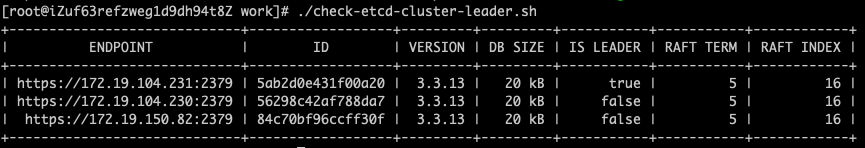
\includegraphics[scale=0.4]{etcd-cluster-leader-view}
	\caption{etcd查看Leader节点}
	\label{fig:etcd-cluster-leader-view}
\end{figure}


\subsubsection{部署master节点}

kubernetes master节点包含的组件如下:\newline

\begin{itemize}
\item {kube-apiserver}
\item {kube-scheduler}
\item{kube-controller-manager}
\end{itemize}

kube-scheduler、kube-controller-manager 和 kube-apiserver 三者的功能紧密相关。同时只能有一个 kube-scheduler、kube-controller-manager 进程处于工作状态,如果运行多个,则需要通过选举产生一个 leader;

\paragraph{下载最新版本的Kubernetes二进制文件}

在中国大陆境内无法直接下载Kubernetes二进制文件,奇怪的是虽然使用了代理,但是还是无法通过dl.k8s.io域名进行下载,没有找到有价值的原因分析。所以此处采取的方式是在国外的主机上下载完毕后,拷贝文件到国内到云主机上进行部署(当然可以下载源码自己编译,不过估计要花不少时间和精力来处理其中遇到的问题),国外主机下载速度较快,在50MB每秒。注意以下命令在国外的服务器上执行,这里是用的美国俄亥俄州的节点,当然香港、新加坡、台湾等物理距离较近的节点更好。

\begin{lstlisting}[language=Bash]
wget -c https://github.com/kubernetes/kubernetes/releases/download/v1.15.2/kubernetes.tar.gz
tar -xzvf kubernetes.tar.gz
cd kubernetes
./cluster/get-kube-binaries.sh
\end{lstlisting}

从Github上下载下来的仅仅是一些脚本,这里下载的是v1.15.2版本的脚本,大概有600KB左右,完整的Binary文件估计有1.5GB+。下载完毕后拷贝到阿里云服务器:

\begin{lstlisting}[language=Bash]
scp -i dolphin.pem -r ubuntu@ec2-23-53-88-011.us-east-2.compute.amazonaws.com:~/* .
\end{lstlisting}

将二进制文件拷贝到指定路径:

\begin{lstlisting}[language=Bash]
cp -r server/bin/{kube-apiserver,kube-controller-manager,kube-scheduler,kubectl,kube-proxy,kubelet} /usr/local/bin/
\end{lstlisting}

\paragraph{配置和启动 kube-apiserver}

kube-apiserver是在部署kubernetes集群是最需要先启动的组件,也是和集群交互的核心组件。创建 kube-apiserver的service配置文件(路径:/usr/lib/systemd/system),service配置文件kube-apiserver.service内容:

\begin{lstlisting}[language=Bash]
[Unit]
Description=Kubernetes API Service
Documentation=https://github.com/GoogleCloudPlatform/kubernetes
After=network.target
After=etcd.service

[Service]
EnvironmentFile=-/etc/kubernetes/config
EnvironmentFile=-/etc/kubernetes/apiserver
ExecStart=/usr/local/bin/kube-apiserver \
        $KUBE_LOGTOSTDERR \
        $KUBE_LOG_LEVEL \
        $KUBE_ETCD_SERVERS \
        $KUBE_API_ADDRESS \
        $KUBE_API_PORT \
        $KUBELET_PORT \
        $KUBE_ALLOW_PRIV \
        $KUBE_SERVICE_ADDRESSES \
        $KUBE_ADMISSION_CONTROL \
        $KUBE_API_ARGS
Restart=on-failure
Type=notify
LimitNOFILE=65536

[Install]
WantedBy=multi-user.target
\end{lstlisting}

/etc/kubernetes/config文件的内容为:

\begin{lstlisting}[language=Bash]
#
# kubernetes system config
#
# The following values are used to 
# configure various aspects of all
# kubernetes services, including
#
#   kube-apiserver.service
#   kube-controller-manager.service
#   kube-scheduler.service
#   kubelet.service
#   kube-proxy.service
# logging to stderr means we get it in the systemd journal
KUBE_LOGTOSTDERR="--logtostderr=true"

# journal message level, 0 is debug
KUBE_LOG_LEVEL="--v=0"

# Should this cluster be allowed 
# to run privileged docker containers
KUBE_ALLOW_PRIV="--allow-privileged=true"

# How the controller-manager, scheduler
# and proxy find the apiserver
KUBE_MASTER="--master=http://172.19.104.231:8080"
\end{lstlisting}

该配置文件同时被kube-apiserver、kube-controller-manager、kube-scheduler、kubelet、kube-proxy使用。添加api server配置文件/etc/kubernetes/apiserver,内容为:

\begin{lstlisting}[language=Bash]
KUBE_API_ADDRESS="--advertise-address=172.19.104.231 --bind-address=172.19.104.231 --insecure-bind-address=172.19.104.231"
#
# The port on the local server to listen on.
#
# Port minions listen on
#
# Comma separated list of nodes in the etcd cluster
KUBE_ETCD_SERVERS="--etcd-servers=https://172.19.104.231:2379,https://172.19.104.230:2379,https://172.19.150.82:2379"
#
# Address range to use for services
KUBE_SERVICE_ADDRESSES="--service-cluster-ip-range=10.254.0.0/16"
#
# default admission control policies
KUBE_ADMISSION_CONTROL="--admission-control=ServiceAccount,NamespaceLifecycle,NamespaceExists,LimitRanger,ResourceQuota"
#
# Add your own!
KUBE_API_ARGS="--authorization-mode=RBAC --runtime-config=rbac.authorization.k8s.io/v1beta1 --kubelet-https=true --enable-bootstrap-token-auth --token-auth-file=/etc/kubernetes/token.csv --service-node-port-range=30000-32767 --tls-cert-file=/etc/kubernetes/ssl/kubernetes.pem --tls-private-key-file=/etc/kubernetes/ssl/kubernetes-key.pem --client-ca-file=/etc/kubernetes/ssl/ca.pem --service-account-key-file=/etc/kubernetes/ssl/ca-key.pem --etcd-cafile=/etc/kubernetes/ssl/ca.pem --etcd-certfile=/etc/kubernetes/ssl/kubernetes.pem --etcd-keyfile=/etc/kubernetes/ssl/kubernetes-key.pem --enable-swagger-ui=true --apiserver-count=3 --audit-log-maxage=30 --audit-log-maxbackup=3 --audit-log-maxsize=100 --audit-log-path=/var/lib/audit.log --event-ttl=1h"
\end{lstlisting}

输入如下命令启动kube-apiserver:

\begin{lstlisting}[language=Bash]
# 调整配置文件后执行此命令重新加载配置
systemctl daemon-reload
systemctl start kube-apiserver.service
systemctl status kube-apiserver.service
\end{lstlisting}

启动kube-apiserver服务时提示unknown flag: --experimental-bootstrap-token-auth,原来Bootstrap Token Authentication在1.9版本已经变成了正式feature(此次部署的版本是v1.15),将kube-apiserver配置文件/etc/kubernetes/apiserver相应参数改为--enable-bootstrap-token-auth即可。启动时提示错误:

\begin{lstlisting}[language=Bash]
clientconn.go:1251] grpc: addrConn.createTransport failed to connect to {172.19.150.82:2379 0  <nil>}. Err :connection error: desc = "transport: authentication handshake failed: x509: certificate signed by unknown authority (possibly because of \"crypto/rsa: verification error\" while trying to verify candidate authority certificate \"kubernetes\")". Reconnecting...
\end{lstlisting}

将pem格式的证书转换为crt格式:

\begin{lstlisting}[language=Bash]
openssl x509 -outform der -in ca.pem -out ca.crt
# 拷贝CA根证书
cp /data/k8s/ssl/ca.crt /etc/pki/ca-trust/source/anchors/
update-ca-trust
\end{lstlisting}

\subsubsection{创建kube-controller-manager集群}

创建证书签名请求:

\begin{lstlisting}[language=Bash]
cd /opt/k8s/work
cat > kube-controller-manager-csr.json <<EOF
{
    "CN": "system:kube-controller-manager",
    "key": {
        "algo": "rsa",
        "size": 2048
    },
    "hosts": [
      "127.0.0.1",
      "172.19.104.230",
      "172.19.104.231",
      "172.19.150.82"
    ],
    "names": [
      {
        "C": "CN",
        "ST": "BeiJing",
        "L": "BeiJing",
        "O": "system:kube-controller-manager",
        "OU": "4Paradigm"
      }
    ]
}
EOF
\end{lstlisting}

hosts列表包含所有 kube-controller-manager节点 IP。创建 kube-controller-manager的serivce配置文件,文件路径/usr/lib/systemd/system/kube-controller-manager.service\footnote{参考链接:\url{https://jimmysong.io/kubernetes-handbook/practice/master-installation.html}}。

\begin{lstlisting}
[Unit]
Description=Kubernetes Controller Manager
Documentation=https://github.com/GoogleCloudPlatform/kubernetes

[Service]
EnvironmentFile=-/etc/kubernetes/config
EnvironmentFile=-/etc/kubernetes/controller-manager
ExecStart=/usr/local/bin/kube-controller-manager \
        $KUBE_LOGTOSTDERR \
        $KUBE_LOG_LEVEL \
        $KUBE_MASTER \
        $KUBE_CONTROLLER_MANAGER_ARGS
Restart=on-failure
LimitNOFILE=65536

[Install]
WantedBy=multi-user.target
\end{lstlisting}

配置文件/etc/kubernetes/controller-manager。

\begin{lstlisting}
###
# The following values are used to configure the kubernetes controller-manager

# defaults from config and apiserver should be adequate

# Add your own!
KUBE_CONTROLLER_MANAGER_ARGS="--address=127.0.0.1 --service-cluster-ip-range=10.254.0.0/16 --cluster-name=kubernetes --cluster-signing-cert-file=/etc/kubernetes/ssl/ca.pem --cluster-signing-key-file=/etc/kubernetes/ssl/ca-key.pem  --service-account-private-key-file=/etc/kubernetes/ssl/ca-key.pem --root-ca-file=/etc/kubernetes/ssl/ca.pem --leader-elect=true"
\end{lstlisting}

通过如下命令启动controller-manager\footnote{来源链接:\url{https://jimmysong.io/kubernetes-handbook/practice/master-installation.html}}:

\begin{lstlisting}[language=Bash]
systemctl start kube-controller-manager
\end{lstlisting}

无法通过服务启动时,可直接通过命令行启动Controller Manager:

\begin{lstlisting}
nohup /usr/local/bin/kube-controller-manager --address=127.0.0.1 --service-cluster-ip-range=10.254.0.0/16 --cluster-name=kubernetes --cluster-signing-cert-file=/etc/kubernetes/ssl/ca.pem --cluster-signing-key-file=/etc/kubernetes/ssl/ca-key.pem  --service-account-private-key-file=/etc/kubernetes/ssl/ca-key.pem --root-ca-file=/etc/kubernetes/ssl/ca.pem --leader-elect=true --master=http://172.19.104.231:8080 &
\end{lstlisting}

\paragraph{配置和启动kube-scheduler}

创建 kube-scheduler的serivce配置文件,文件路径/usr/lib/systemd/system/kube-scheduler.service。使用命令行启动kubernetes scheduler:

\begin{lstlisting}[language=Bash]
/usr/local/bin/kube-scheduler --master=http://172.19.104.231:8080 --leader-elect=true --address=127.0.0.1
\end{lstlisting}


\paragraph{验证master节点功能}

master所有组件启动完成后,使用如下命令查看组件状态:

\begin{lstlisting}[language=Bash]
kubectl get componentstatuses
\end{lstlisting}

提示错误:The connection to the server localhost:8080 was refused - did you specify the right host or port?此错误表示kubectl未正确配置。配置kubeconfig如下:

\begin{lstlisting}[language=Bash]
export KUBE_APISERVER="http://172.19.104.231:8080"
# 设置集群参数
kubectl config set-cluster kubernetes \
  --certificate-authority=/etc/kubernetes/ssl/ca.pem \
  --embed-certs=true \
  --server=${KUBE_APISERVER}
# 设置客户端认证参数
kubectl config set-credentials admin \
  --client-certificate=/etc/kubernetes/ssl/admin.pem \
  --embed-certs=true \
  --client-key=/etc/kubernetes/ssl/admin-key.pem
# 设置上下文参数
kubectl config set-context kubernetes \
  --cluster=kubernetes \
  --user=admin
# 设置默认上下文
kubectl config use-context kubernetes
\end{lstlisting}

添加部分基础配置后,连接拒绝的错误消失。输出各个组件的状态(Component Status):

\begin{lstlisting}
NAME                 STATUS    MESSAGE             ERROR
scheduler            Healthy   ok
controller-manager   Healthy   ok
etcd-1               Healthy   {"health":"true"}
etcd-0               Healthy   {"health":"true"}
etcd-2               Healthy   {"health":"true"}
\end{lstlisting}

\subsubsection{安装flannel网络插件}

覆盖网络(Overlay Network)就是应用层网络,它是面向应用层的,不考虑或很少考虑网络层,物理层的问题。详细说来,覆盖网络是指建立在另一个网络上的网络。该网络中的结点可以看作通过虚拟或逻辑链路而连接起来的。虽然在底层有很多条物理链路,但是这些虚拟或逻辑链路都与路径一一对应。例如:许多P2P网络就是覆盖网络,因为它运行在互连网的上层。覆盖网络允许对没有IP地址标识的目的主机路由信息,例如:Freenet 和DHT(分布式哈希表)可以路由信息到一个存储特定文件的结点,而这个结点的IP地址事先并不知道。覆盖网络被认为是一条用来改善互连网路由的途径,让二层网络在三层网络中传递,既解决了二层的缺点,又解决了三层的不灵活!Flannel实质上是一种“覆盖网络(overlay network)”,也就是将TCP数据包装在另一种网络包里面进行路由转发和通信,目前已经支持UDP、VxLAN、AWS VPC和GCE路由等数据转发方式。数据从源容器中发出后,经由所在主机的docker0虚拟网卡转发到flannel0虚拟网卡,这是个P2P的虚拟网卡,flanneld服务监听在网卡的另外一端。Flannel通过Etcd服务维护了一张节点间的路由表,详细记录了各节点子网网段 。源主机的flanneld服务将原本的数据内容UDP封装后根据自己的路由表投递给目的节点的flanneld服务,数据到达以后被解包,然后直接进入目的节点的flannel0虚拟网卡,然后被转发到目的主机的docker0虚拟网卡,最后就像本机容器通信一下的有docker0路由到达目标容器。所有的node节点都需要安装网络插件才能让所有的Pod加入到同一个局域网中,本文是安装flannel网络插件的参考文档。

\paragraph{下载分发flannel二进制文件}

获取flannel部署文件\footnote{来源链接:\url{https://github.com/opsnull/follow-me-install-kubernetes-cluster/blob/master}}:

\begin{lstlisting}[language=Bash]
cd /opt/k8s/work
mkdir flannel
wget https://github.com/coreos/flannel/releases/download/v0.11.0/flannel-v0.11.0-linux-amd64.tar.gz
tar -xzvf flannel-v0.11.0-linux-amd64.tar.gz -C flannel
\end{lstlisting}

service配置文件/usr/lib/systemd/system/flanneld.service。

\begin{lstlisting}
[Unit]
Description=Flanneld overlay address etcd agent
After=network.target
After=network-online.target
Wants=network-online.target
After=etcd.service
Before=docker.service

[Service]
Type=notify
EnvironmentFile=/etc/sysconfig/flanneld
EnvironmentFile=-/etc/sysconfig/docker-network
ExecStart=/usr/bin/flanneld-start \
  -etcd-endpoints=${FLANNEL_ETCD_ENDPOINTS} \
  -etcd-prefix=${FLANNEL_ETCD_PREFIX} \
  $FLANNEL_OPTIONS
ExecStartPost=/usr/libexec/flannel/mk-docker-opts.sh -k DOCKER_NETWORK_OPTIONS -d /run/flannel/docker
Restart=on-failure

[Install]
WantedBy=multi-user.target
RequiredBy=docker.service
\end{lstlisting}

/etc/sysconfig/flanneld配置文件:

\begin{lstlisting}
# Flanneld configuration options  

# etcd url location.  Point this to the server where etcd runs
FLANNEL_ETCD_ENDPOINTS="https://172.19.104.231:2379,https://172.19.104.230:2379,https://172.19.150.82:2379"

# etcd config key.  This is the configuration key that flannel queries
# For address range assignment
FLANNEL_ETCD_PREFIX="/kube-centos/network"

# Any additional options that you want to pass
FLANNEL_OPTIONS="-etcd-cafile=/etc/kubernetes/ssl/ca.pem -etcd-certfile=/etc/kubernetes/ssl/kubernetes.pem -etcd-keyfile=/etc/kubernetes/ssl/kubernetes-key.pem"
\end{lstlisting}

执行下面的命令为docker分配IP地址段。

\begin{lstlisting}[language=Bash]
etcdctl --endpoints=https://172.19.104.231:2379,https://172.19.104.230:2379,https://172.19.150.82:2379 \
  --ca-file=/etc/kubernetes/ssl/ca.pem \
  --cert-file=/etc/kubernetes/ssl/kubernetes.pem \
  --key-file=/etc/kubernetes/ssl/kubernetes-key.pem \
  mkdir /kube-centos/network
etcdctl --endpoints=https://172.19.104.231:2379,https://172.19.104.230:2379,https://172.19.150.82:2379 \
  --ca-file=/etc/kubernetes/ssl/ca.pem \
  --cert-file=/etc/kubernetes/ssl/kubernetes.pem \
  --key-file=/etc/kubernetes/ssl/kubernetes-key.pem \
  mk /kube-centos/network/config '{"Network":"172.30.0.0/16","SubnetLen":24,"Backend":{"Type":"vxlan"}}'
\end{lstlisting}

启动flannel:

\begin{lstlisting}[language=Bash]
systemctl daemon-reload
systemctl enable flanneld
systemctl start flanneld
systemctl status flanneld
\end{lstlisting}

也可直接执行如下命令启动:

\begin{lstlisting}[language=Bash]
/usr/bin/flanneld -etcd-endpoints=https://172.19.104.231:2379,https://172.19.104.230:2379,https://172.19.150.82:2379 -etcd-prefix=/kube-centos/network -etcd-cafile=/etc/kubernetes/ssl/ca.pem -etcd-certfile=/etc/kubernetes/ssl/kubernetes.pem -etcd-keyfile=/etc/kubernetes/ssl/kubernetes-key.pem
/root/flanneld -etcd-endpoints=https://172.19.104.231:2379,https://172.19.104.230:2379,https://172.19.150.82:2379 -etcd-prefix=/kube-centos/network -etcd-cafile=/etc/kubernetes/ssl/ca.pem -etcd-certfile=/etc/kubernetes/ssl/kubernetes.pem -etcd-keyfile=/etc/kubernetes/ssl/kubernetes-key.pem
\end{lstlisting}

启动时提示错误:failed to retrieve network config: 100: Key not found (/kube-centos)。要先设置key:

\begin{lstlisting}[language=Bash]
# v2版本写法
etcdctl set /kube-centos/network/config '{ "Network":"10.1.0.0/16" }'
# v3版本写法
etcdctl put /kube-centos/network/config '{ "Network":"10.1.0.0/16" }'
etcdctl get /kube-centos/network/config
# 查看所有的key(etcd v3写法)
etcdctl get / --prefix --keys-only
# 查看集群信息
ETCDCTL_API=3 etcdctl get /registry/pods --prefix -w json|python -m json.tool
\end{lstlisting}

实际操作过程中,即使设置好了key,也还是会抛出Key not found的异常,初步确定是由于flannel截止到2019年09月06日,还没有兼容分布式数据库etcd v3版本,读取分布式数据库还是采用的v2版本的读取方式,而v3版本和v2版本的读取方式是不兼容的,所以会出现数据库明明已经设置了对应的key,但是flannel还是始终无法读取到,提示key未找到错误。Etcd V2和V3之间的数据结构完全不同,互不兼容,也就是说使用V2版本的API创建的数据只能使用V2的API访问,V3的版本的API创建的数据只能使用V3的API访问。这就造成我们访问etcd中保存的flannel的数据需要使用etcdctl的V2版本的客户端,而访问kubernetes的数据需要设置ETCDCTL\_API=3环境变量来指定V3版本的API。安装好flannel插件后,可以在etcd中检查是否有相应的数据,来判断是否运行正常。查询etcd中的内容可以看到:

\begin{lstlisting}[language=Bash]
/usr/local/bin/etcdctl --endpoints=${ETCD_ENDPOINTS} \
--cacert=/etc/kubernetes/ssl/ca.pem \
--cert=/etc/kubernetes/ssl/kubernetes.pem \
--key=/etc/kubernetes/ssl/kubernetes-key.pem \
\end{lstlisting}

注意不同版本的etcdctl其命令的参数有可能不一致,此处使用的etcdctl版本是3.3.13。

\paragraph{安装完毕后验证}

在各节点上部署 flannel 后,检查是否创建了 flannel 接口(名称可能为 flannel0、flannel.0、flannel.1 等):

\begin{lstlisting}[language=Bash]
source /opt/k8s/bin/environment.sh
for node_ip in ${NODE_IPS[@]}
  do
    echo ">>> ${node_ip}"
    ssh ${node_ip} "/usr/sbin/ip addr show flannel.1|grep -w inet"
  done
\end{lstlisting}

输出的内容如下:

\begin{lstlisting}
>>> 172.19.104.231
    inet 172.30.224.0/32 scope global flannel.1
>>> 172.19.104.230
    inet 172.30.208.0/32 scope global flannel.1
>>> 172.19.150.82
    inet 172.30.184.0/32 scope global flannel.1
\end{lstlisting}

在各节点上 ping 所有 flannel 接口 IP,确保能通:

\begin{lstlisting}[language=Bash]
source /opt/k8s/bin/environment.sh
for node_ip in ${NODE_IPS[@]}
  do
    echo ">>> ${node_ip}"
    ssh ${node_ip} "ping -c 1 172.30.80.0"
    ssh ${node_ip} "ping -c 1 172.30.32.0"
    ssh ${node_ip} "ping -c 1 172.30.184.0"
  done
\end{lstlisting}

此脚本会登陆各台主机,分别ping所有主机,保证所有主机之间能够互相ping通。在安装的过程中,遇到了本主机的IP可以ping通,但是其他主机的IP无法ping通的情况。添加iptables规则解决此问题(实际上主机的iptables服务是没有启动的):

\begin{lstlisting}[language=Bash]
sudo iptables -P INPUT ACCEPT
sudo iptables -P OUTPUT ACCEPT
sudo iptables -P FORWARD ACCEPT
\end{lstlisting}

由于82这台主机使用的是firewalld防火墙,暂时还不清楚flannel服务需要开启哪个端口才可以正常访问,暂时开启所有端口来解决部署问题:

\begin{lstlisting}[language=Bash]
firewall-cmd --permanent --zone=public --add-port=0-65525/tcp
firewall-cmd --permanent --zone=public --add-port=0-65535/udp
firewall-cmd --reload
\end{lstlisting}

\subsection{部署 kubelet 组件}

\subsubsection{创建和分发kubelet systemd unit文件}

创建kubelet systemd unit文件模板,创建模版时,检查启动命令不要有allow-privileged参数,由于此处部署的是Kubernetes v1.15.2版本,allow-privileged已经在1.15.0版本中删除\footnote{内容来源:\url{https://github.com/opsnull/follow-me-install-kubernetes-cluster/blob/master/07-2.kubelet.md}}:

\begin{lstlisting}
cd /opt/k8s/work
source /opt/k8s/bin/environment.sh
cat > kubelet.service.template <<EOF
[Unit]
Description=Kubernetes Kubelet
Documentation=https://github.com/GoogleCloudPlatform/kubernetes
After=docker.service
Requires=docker.service

[Service]
WorkingDirectory=${K8S_DIR}/kubelet
ExecStart=/opt/k8s/bin/kubelet \\
  --bootstrap-kubeconfig=/etc/kubernetes/kubelet-bootstrap.kubeconfig \\
  --cert-dir=/etc/kubernetes/cert \\
  --cni-conf-dir=/etc/cni/net.d \\
  --container-runtime=docker \\
  --container-runtime-endpoint=unix:///var/run/dockershim.sock \\
  --root-dir=${K8S_DIR}/kubelet \\
  --kubeconfig=/etc/kubernetes/kubelet.kubeconfig \\
  --config=/etc/kubernetes/kubelet-config.yaml \\
  --hostname-override=##NODE_NAME## \\
  --pod-infra-container-image=registry.cn-beijing.aliyuncs.com/images_k8s/pause-amd64:3.1 \\
  --image-pull-progress-deadline=15m \\
  --volume-plugin-dir=${K8S_DIR}/kubelet/kubelet-plugins/volume/exec/ \\
  --logtostderr=true \\
  --v=2
Restart=always
RestartSec=5
StartLimitInterval=0

[Install]
WantedBy=multi-user.target
EOF
\end{lstlisting}

\subsubsection{启动kubelet服务}

如下指令启动kubelet服务:

\begin{lstlisting}[language=Bash]
source /opt/k8s/bin/environment.sh
for node_ip in ${NODE_IPS[@]}
  do
    echo ">>> ${node_ip}"
    ssh root@${node_ip} "mkdir -p ${K8S_DIR}/kubelet/kubelet-plugins/volume/exec/"
    ssh root@${node_ip} "/usr/sbin/swapoff -a"
    ssh root@${node_ip} "systemctl daemon-reload && systemctl enable kubelet && systemctl restart kubelet"
  done
\end{lstlisting}

kubelet启动后使用--bootstrap-kubeconfig向kube-apiserver发送CSR(Certificate Signing Request)请求,当这个CSR被 approve 后,kube-controller-manager 为 kubelet 创建 TLS 客户端证书、私钥和 --kubeletconfig 文件。注意:kube-controller-manager 需要配置 --cluster-signing-cert-file 和 --cluster-signing-key-file 参数,才会为 TLS Bootstrap 创建证书和私钥。启动时提示错误:unknown flag: --allow-privileged,是由于kubelet 1.15.0的启动参数中allow-privileged已被删除,所以在启动参数中将之移除。

\subsubsection{查看kubelet的情况}

等待一段时间(1-10 分钟),三个节点的CSR都被自动 approved:

\begin{lstlisting}[language=Bash]
/opt/k8s/bin/kubectl get csr
\end{lstlisting}

如果执行命令提示No resources found,则可以使用如下命令查看kubelet服务运行日志:

\begin{lstlisting}[language=Bash]
systemctl status kubelet -l
systemctl status kubelet.service | tail 
\end{lstlisting}

提示错误Failed to list *v1.Pod: Unauthorized。第一确认kube-apiserver的确配置了Node授权模式: --authorization-mode=Node,RBAC。/etc/kubernetes/cert/目录下有kubelet-client 和 kubelet-server证书。kubelet 启动时查找 --kubeletconfig 参数对应的文件是否存在,如果不存在则使用 --bootstrap-kubeconfig 指定的 kubeconfig 文件向 kube-apiserver 发送证书签名请求 (CSR)。kube-apiserver 收到 CSR 请求后,对其中的 Token 进行认证,认证通过后将请求的 user 设置为 system:bootstrap:<Token ID>,group 设置为 system:bootstrappers,这一过程称为 Bootstrap Token Auth。默认情况下,这个 user 和 group 没有创建 CSR 的权限,kubelet 启动失败。解决办法是:创建一个 clusterrolebinding,将 group system:bootstrappers 和 clusterrole system:node-bootstrapper 绑定:

\begin{lstlisting}[language=Bash]
/opt/k8s/bin/kubectl create clusterrolebinding kubelet-bootstrap --clusterrole=system:node-bootstrapper --group=system:bootstrappers
\end{lstlisting}

执行完毕以上动作,查看集群CSR(Certificate Signing Request)时,输出如下内容:

\begin{lstlisting}[language=Bash]
[root@ops001 work]# kubectl get csr
NAME        AGE     REQUESTOR                 CONDITION
csr-2k5rp   8m9s    system:bootstrap:6o33uh   Pending
csr-4q7qw   23m     system:bootstrap:27qa60   Pending
csr-4rtpz   4m57s   system:bootstrap:58ndy6   Pending
csr-92bs9   8m8s    system:bootstrap:27qa60   Pending
csr-c8gql   23m     system:bootstrap:6o33uh   Pending
csr-csxnq   23m     system:bootstrap:58ndy6   Pending
csr-dr6ld   23m     system:bootstrap:27qa60   Pending
csr-hcppn   23m     system:bootstrap:58ndy6   Pending
csr-k6khk   23m     system:bootstrap:6o33uh   Pending
csr-t4xk7   19m     system:bootstrap:58ndy6   Pending
\end{lstlisting}

可以看出当前所有的CSR都处于Pending状态,需要注意的是,在查看CSR的时候,由于生成CSR需要较长时间,当前输出的可能是部分需要approve的CSR,根据实际经验,即使在手动approve到最后的CSR时,仍然会有新的CSR产生。

\subsubsection{手动Approve Server Certificate CSR}

基于安全性考虑,CSR approving controllers 不会自动 approve kubelet server 证书签名请求,需要手动approve,输入如下命令手动Approval证书:

\begin{lstlisting}[language=Bash]
/opt/k8s/bin/kubectl certificate approve csr-2k5rp
\end{lstlisting}

\subsection{部署CoreDNS插件}

CoreDNS 是一个 Go 语言实现的链式插件,是一个高性能、易扩展的 DNS 服务端。集群中的每个流程都需要知道自己是如何与其他服务联系,但集群 IP 地址往往是动态的,很难通过 IP 来解决服务问题。CoreDNS 为服务提供了一种发现彼此的方式,开发者只需知道服务名称,CoreDNS 就可回复相应 IP地址。CoreDNS在Kubernetes1.11版本已经做为GA功能释放,成为Kubernetes默认的DNS服务替代了Kube-DNS,目前是kubeadm、kube-up、minikube和kops安装工具的默认选项。kuberntes自带插件的 manifests yaml 文件使用 gcr.io 的 docker registry,国内被墙,需要手动替换为其它registry地址,这里替换成了微软中国镜像\footnote{镜像地址:\url{http://mirror.azk8s.cn},其中GCR Proxy Cache服务帮助地址:\url{http://mirror.azk8s.cn/help/gcr-proxy-cache.html},截止到2019年09月20日,该地址可以正常访问。}地址(微软提供镜像服务确实很赞,又多了一个选择,如果是过去几年微软提供镜像部署Google的服务是不大可能的),例如CoreDNS的地址是gcr.azk8s.cn/google-containers/coredns:1.3.1,替换CoreDNS地址后,可以使用如下命令验证地址是否可用:

\begin{lstlisting}[language=Bash]
# 测试Kubenetes Dashboard镜像地址是否可达
docker pull gcr.azk8s.cn/google_containers/kubernetes-dashboard-amd64:v1.10.1
# 测试CoreDNS镜像地址是否可达
docker pull gcr.azk8s.cn/google-containers/coredns:1.3.1
\end{lstlisting}

调整CoreDNS配置文件(/opt/k8s/work/kubernetes/cluster/addons/dns/coredns),需要将\_\_PILLAR\_\_DNS\_\_DOMAIN\_\_设置为集群环境中的域名, 这个域名需要和kubelet的--cluster-domain参数值一致。查看集群的cluster Domain在配置文件/etc/kubernetes/kubelet-config.yaml中,显示的是cluster.local。需要将\_\_PILLAR\_\_DNS\_\_SERVER\_\_设置为集群环境的IP, 这个IP需要和kubelet的--cluster-dns参数值一致,kubelet的cluster DNS配置也在kubelet config文件中,值是10.254.0.2。使用如下命令部署CoreDNS:

\begin{lstlisting}[language=Bash]
kubectl create -f coredns.yaml
\end{lstlisting}

\subsection{安装Kubernetes Dashboard插件}

Kubernetes的国外安装其实非常简单,国内安装的主要问题在于kubernetes部件所需的官方镜像在 http://gcr.io(Google Cloud Container Registry)上,但是此网站在国内是无法访问的。当前安装Kubernetes Dashboard的时间是2019年08月30日,本文档中安装的是kubernetes dashboard v1.6.0\footnote{参考来源:\url{https://jimmysong.io/kubernetes-handbook/practice/dashboard-addon-installation.html}}。执行如下命令部署Dashboard Web UI(此方法不可取,在实际部署过程中,由于国内特殊的网络环境,部署所需要的部分镜像无法获取,在部署之前,还需要修改部分镜像的地址配置,将地址修改为国内网络可以访问的地址\footnote{具体可以参考文章:\url{https://jimmysong.io/kubernetes-handbook/practice/dashboard-upgrade.html}},方可继续部署,否则后面需要花费大量的事件处理各种莫名的问题,浪费时间和精力):

\begin{lstlisting}[language=Bash]
# 安装Dashboard
kubectl apply -f https://raw.githubusercontent.com/kubernetes/dashboard/v1.10.1/src/deploy/recommended/kubernetes-dashboard.yaml
# 卸载Dashboard
kubectl delete -f https://raw.githubusercontent.com/kubernetes/dashboard/v1.10.1/src/deploy/recommended/kubernetes-dashboard.yaml
\end{lstlisting}

部署完毕后,查看Pods:

\begin{lstlisting}[language=Bash]
kubectl get pod --namespace=kube-system
# 查看所有命名空间的Pods
kubectl get pods --all-namespaces
kubectl get pods,svc --all-namespaces -o wide
\end{lstlisting}

查看到镜像一直处于Pending状态,查看镜像的日志:

\begin{lstlisting}[language=Bash]
kubectl --namespace kube-system logs kubernetes-dashboard-7d75c474bb-b2lwd
# 查看Dashboard对外映射的端口
kubectl get svc -n kube-system
\end{lstlisting}

如果日志没有输出,查看事件:

\begin{lstlisting}[language=Bash]
kubectl get events --namespace=kube-system
\end{lstlisting}

通过事件可以看出kube-dns和metrics-server服务IP范围指定与原有的IP范围不一致,提示ClusterIPOutOfRange错误。查看镜像的配置:

\begin{lstlisting}[language=Bash]
./kubectl describe pod kubernetes-dashboard-7d75c474bb-b2lwd --namespace="kube-system"
\end{lstlisting}

启动Scheduler组件时,提示Failed to update lock: Operation cannot be fulfilled on endpoints "kube-scheduler": StorageError: invalid object, Code: 4, Key: /registry/services/endpoints/kube-system/kube-scheduler, ResourceVersion: 0, AdditionalErrorMsg: Precondition failed: UID in precondition: 121bc661-80f5-11e9-b3ce-00163e086f0c, UID in object meta: 49e84916-589a-4da5-b78a-761a1fe78285错误。

查看集群信息:

\begin{lstlisting}[language=Bash]
# 查看集群IP信息
kubectl cluster-info dump | grep service-cluster-ip-range
kubectl get cm kubeadm-config -n kube-system -o yaml
\end{lstlisting}


\subsubsection{通过代理访问dashboard}

可以使用 kubectl 命令行工具访问 Dashboard,启动代理命令如下:

\begin{lstlisting}[language=Bash]
kubectl proxy --address=0.0.0.0 --port=8001 --accept-hosts='^*$'
\end{lstlisting}

accept-hosts设置API接收所有主机的请求。输入如下链接通过kubectl proxy访问Dashboard:

\begin{lstlisting}[language=Bash]
curl http://172.19.150.82:8001/api/v1/namespaces/kube-system/services/https:kubernetes-dashboard:/proxy/
http://kubernetes.example.com/api/v1/namespaces/kube-system/services/kube-ui/#/dashboard/
curl http://172.19.104.231:8001/api/v1/proxy/namespaces/kube-system/services/kubernetes-dashboard/
# 通过域名访问的访问地址
# 不过返回的Json字符串
https://kubernetes.ttt208.com/api/v1/namespaces/kube-system/services/kubernetes-dashboard
\end{lstlisting}

需要注意的是,Kubernetes Web UI默认只支持在直接执行代理操作命令的机器上访问。查看kube-system命名空间下pod状态:

\begin{lstlisting}[language=Bash]
kubectl get pod --namespace=kube-system
\end{lstlisting}

访问Kubenetes Dashboard时提示no endpoints available for service "kubernetes-dashboard"。

\begin{lstlisting}[language=Bash]
kubectl get pods --namespace kube-system
kubectl describe pod kubernetes-dashboard-74d7cc788-mk9c7 --namespace kube-system
kubectl logs -n kube-system kubernetes-dashboard-74d7cc788-mk9c7 -c dnsmasq
\end{lstlisting}

发现问题是no nodes available to schedule pods,无可用节点,原来是没有安装kubelet组件导致,安装组件将节点修复即可。

\subsubsection{通过kube-apiserver访问Dashboard}

\begin{lstlisting}[language=Bash]
https://172.19.104.231:6443/api/v1/namespaces/kube-system/services/https:kubernetes-dashboard:/proxy
\end{lstlisting}

在公网访问Dashboard链接:

\begin{lstlisting}[language=Bash]
http://kubernetes.ttt208.com/api/v1/namespaces/kube-system/services/https:kubernetes-dashboard:/proxy/
http://172.19.104.231:8001/api/v1/namespaces/kube-system/services/https:kubernetes-dashboard:/proxy/
http://172.19.150.82:8001/api/v1/namespaces/kube-system/services/https:kubernetes-dashboard:/proxy/
curl -L http://172.19.150.82:31085/ui
\end{lstlisting}

提示错误:Error: 'dial tcp 172.17.0.6:8443: connect: connection refused',Trying to reach: 'https://172.17.0.6:8443/'。在主机172.19.104.231上可以ping通此IP,使用如下命令列出主机172.19.104.231所有IP:

\begin{lstlisting}[language=Bash]
docker inspect --format='{{.Name}} - {{range .NetworkSettings.Networks}}{{.IPAddress}}{{end}}' $(docker ps -aq)
\end{lstlisting}

输出结果如下:

\begin{lstlisting}[language=Bash]
/elegant_rosalind - 172.17.0.10
/confluence - 172.17.0.5
/gitlab - 172.17.0.2
/nexus3 - 172.17.0.9
/jenkins - 172.17.0.6
/mysql_atlassian - 172.17.0.7
/jira - 172.17.0.8
/nginx - 172.17.0.4
/rancher-server - 172.17.0.3
\end{lstlisting}

说明访问Dashboard UI时,系统指向了主机上jenkins的容器地址,jenkins容器自然没有启动8443端口,所以会提示错误。而登陆Dashboard部署的主机查看,刚好发现Dashboard容器的IP也是172.17.0.6,说明不同主机的Docker分配到了相同的IP,这就是一个跨主机容器IP冲突的问题了。尝试将Jenkins的IP重新获取,避免和Kubernetes容器的IP冲突,发现也无法解决问题。经过分析,各个主机的IP无法联通,本质上还是属于跨主机容器通信的问题。为什么会产生这样的问题?是由于Kubernetes是后来部署的,在部署flannel网络组件之前,主机上已经启动了Docker并部署了其他应用,后来在加入flannel组件时,原来的应用没有纳入flannel的网络管理,而从公网访问Kubernetes集群又由早先部署在Docker中的Nginx应用转发,Nginx和Dashboard分别部署在不同主机的Docker中,在没有采用flannel做跨主机容器通信之前,Nginx当然无法访问后来新增的Kubernetes Dashboard。所以尝试将不同主机的Docker纳入flannel统一分配网段,才是解决问题的根本办法。

\subsubsection{Docker加入Flannel网络}

如果需要跨主机容器间能够通信,考虑将原有的Docker容器加入到flannel网络中。Docker安装完成以后,需要修改其启动参数以使其能够使用flannel进行IP分配,以及网络通讯。在flannel运行之后,主要做了以下几步的工作:从etcd中获取network的配置信息;划分subnet,并在etcd中进行注册;将子网信息记录到/run/flannel/subnet.env中。生成一个环境变量文件,包含了当前主机要使用flannel通讯的相关参数,如下:

\begin{lstlisting}[language=Bash]
[root@ops001 conf.d]# cat /run/flannel/subnet.env
FLANNEL_NETWORK=172.30.0.0/16
FLANNEL_SUBNET=172.30.224.1/21
FLANNEL_MTU=1450
FLANNEL_IPMASQ=true
\end{lstlisting}

最大传输单元(Maximum Transmission Unit,MTU)是指一种通信协议的某一层上面所能通过的最大数据报大小(以字节为单位)。IP Masquerade 是 Linux 發展中的一種網路功能.如果一台 Linux 主機使用 IP Masquerade 功能連線到網際網路上,那麼接上它的電腦(不論是在同一個區域網路上或藉由數據機連線)也可以接觸網際網路,即使它們沒有獲得正式指定的 IP 位址.這使得一些電腦可以隱藏在閘道(gateway) 系統後面存取網際網路而不被發現,看起來就像只有這個系統在使用網際網路.突破設定良好的偽裝(masquerade)系統之安全防護應該會比突破良好的封包過濾式防火牆(packet filter firewall)來得更加困難\footnote{内容来源:\url{http://www.e-infomax.com/ipmasq/howto-trans/zh/ipmasq-HOWTO-zh-2.html}}.输入如下命令将subnet.env转写成Docker启动参数,创建好的启动参数默认生成在/run/docker\_opts.env文件中:

\begin{lstlisting}[language=Bash]
[root@ops001 conf.d] cat /run/docker_opts.env
DOCKER_OPTS=" --bip=172.30.224.1/21 --ip-masq=false --mtu=1450"
\end{lstlisting}

修改docker的服务启动文件如下:

\begin{lstlisting}[language=Bash]
# vim /lib/systemd/system/docker.service

EnvironmentFile=/run/docker_opts.env
ExecStart=/usr/bin/dockerd $DOCKER_OPTS -H fd://
\end{lstlisting}

重启Docker,这时可以看到docker0的ip已经位于flannel网卡的网段之中。

\subsection{集群状态检查}

查看所有节点:

\begin{lstlisting}[language=Bash]
# 查看pods
/opt/k8s/bin/kubectl get pods
# 查看集群健康状态
/opt/k8s/bin/kubectl get cs -o wide
# 查看kube-apiserver日志
journalctl -f -u kube-apiserver
kubectl logs kubernetes-dashboard-74d7cc788-mk9c7 -n kube-system
\end{lstlisting}




%----------------------------------------------------------------------------------------
%	BIBLIOGRAPHY
%----------------------------------------------------------------------------------------

\chapter*{Bibliography}
\addcontentsline{toc}{chapter}{\textcolor{ocre}{Bibliography}}
\section*{Books}
\addcontentsline{toc}{section}{Books}
%\printbibliography[heading=bibempty,type=book]
\section*{Articles}
\addcontentsline{toc}{section}{Articles}
%\printbibliography[heading=bibempty,type=article]

%----------------------------------------------------------------------------------------
%	INDEX
%----------------------------------------------------------------------------------------

\cleardoublepage
\phantomsection
\setlength{\columnsep}{0.75cm}
\addcontentsline{toc}{chapter}{\textcolor{ocre}{Index}}
\printindex

%----------------------------------------------------------------------------------------

\end{document}


